\newcommand{\CLASSINPUTinnersidemargin}{0.7in}
\newcommand{\CLASSINPUToutersidemargin}{0.7in}
\documentclass{article}

\usepackage{graphicx}
\usepackage{multirow}

\usepackage{url} % to include URLs in bib entries

\title{Optimizing and Modeling Dynamics in Networks}
\author{{\sc Ibrahim Matta} \\
Computer Science Department \\
Boston University \\
Boston, MA 02215, USA}
\date{\today}							% Activate to display a given date or no date

\def\pd#1#2{\frac{\partial#1}{\partial#2}}   % my own macros
\def\lg{{\rm log}}
\def\L{{\cal L}}
\def\sn{{\rm sin}}
\def\cs{{\rm cos}}
\def\lm{{\rm lim}}
\newcommand{\Conv}{\mathop{\scalebox{1.5}{\raisebox{-0.2ex}{$\ast$}}}}%
\def\junk#1{}


\begin{document}
\maketitle

\tableofcontents

%%%%%
\section{Introduction}

The Internet has grown very large. No one knows exactly how large, but rough estimates indicate billions of users (around 1.8B in 2009, according to eTForecasts \cite{eTForecasts}), hundreds of millions of web sites (over 200M in February 2009, according to Netcraft \cite{Netcraft}), and hundreds of billions of web pages (over 240B, according to the Internet archive \cite{Internet-archive}).
The Internet is also very dynamic --- users log in and out, new services get added, routing policies change, normal traffic gets mixed with denial-of-service (DoS) attack traffic, etc.

An important question is: {\em How do we manage such a huge and highly dynamic structure like the Internet?}
As a corollary, how can we build a network of the future unless we understand the {\em steady-state} and {\em dynamics} of what we build?

In this chapter, we resort to two mathematical frameworks: {\em optimization theory} to study optimal steady states of networks, and {\em control theory} to study the dynamic behavior of networks as they evolve toward steady state. Our emphasis will be on {\em congestion control} using the notion of {\em prices} to model the level of congestion, such as delays and losses, observed by users or traffic sources.

\paragraph{Expected Background:} We assume basic background in calculus and algebra.
We also assume basic knowledge of systems modeling, optimization theory, Laplace transforms, and control theory --- Keshav's textbook \cite{Keshav:2010} provides an excellent source for these mathematical foundations,
in particular, chapters 4, 5, and 8.
Basic knowledge of Internet's Transmission Control Protocol (TCP) \cite{tcp:1988},
namely Reno and Vegas \cite{vegas:1995} versions,
as well as queue management schemes, namely Random Early Drop (RED) \cite{red:1993},
should be helpful.
This chapter briefly covers needed background material to serve as a refresher or quick reference.
The material of this chapter has been used at Boston University in a second (advanced) networking course
taken by senior undergraduate and graduate students.


\paragraph{Contribution and Outline:}
The purpose of this chapter is to make the application of optimization and control theory to congestion control
more accessible through intuitive explanations and simple control applications, 
using examples from Internet's protocols.
This chapter has been largely influenced by the work of Frank Kelly \cite{Kelly-2001}, 
which introduces the notion of ``prices" and ``user utility",
the work by R. Srikant \cite{Srikant:2004},
which discusses the dynamics of user (traffic source) and network adaptations,
and control theory texts and notes (e.g., \cite{Ogata:2010,Lu:2001}). 
The exposition here attempts to tie these various mathematical models and techniques
through simple running examples and illustrations, 
modeling the dynamics of both flow control and routing.
 
We start by motivating the network control problem using analogy to 
the problem of producing, pricing, and consuming gas/oil (Section~\ref{sec:optimization}).
We introduce several examples of optimally allocating resources (link bandwidth) to users (traffic sources),
resulting in different notions of fairness. 
We then introduce dynamic equations that model source and link adaptation algorithms (Section~\ref{sec:control}).
Since these are generally non-linear equations,
we review the technique of linearization and how classical (linear) control theory can be used
to study stability and transient performance (Section~\ref{sec:linear}).
We use as a running example, a Vegas-like system controlled using different types of well-established controllers. 
Using linear approximation around a certain operating point, 
we can only study so-called {\em local} stability.

To study general ({\em global}) stability of non-linear models, 
we introduce the control-theoretic Lyapunov method (Section~\ref{sec:nonlinear}).
We also show how the control-theoretic Nyquist stability method can be applied
to the linearized model to study the impact of delay in feedback (i.e., measurements of the current state of the system).
The material on the Nyquist method is a bit more advanced and can be skipped on a first reading.
We generalize the notion of stability by introducing the concept of contractive mapping,
and extend its application to routing dynamics (Section~\ref{sec:routing}).

Finally, 
we provide two case studies that apply control-theoretic techniques introduced in this chapter:
the first study investigates stability under class-based scheduling
of rate-adaptive traffic flows (Section~\ref{sec:case1}),
and the second study investigates stability of data transfer over 
a dynamic number of rate-adaptive transport connections (Section~\ref{sec:case2}).
These case studies can be skipped on a first reading.

The chapter concludes with a set of exercises (Section~\ref{sec:exercises})
and their solutions  (Section~\ref{sec:solutions}).

%%%%%
\section{Network Control as an Optimization Problem} 
\label{sec:optimization}

In this section, we describe Frank Kelly's optimization framework \cite{Kelly-2001}, which models users' expectations (requirements) with utility functions, and network congestion signals (e.g., loss, delay) as prices. The network is shown to allocate transmission rates (throughputs) to users (flows) in such a way as to meet some {\em fairness} objective.
 
The objective of a user, or what makes the user happy, can be mathematically modeled as a {\em utility function}. For example, drivers observe the``price" of transportation and make one of many possible decisions: drive, take the subway instead, walk, bike, or stay home. The decision may involve several factors like the price of gas, convenience, travel time, etc. 
For example, if it rains, you might decide to drive to work, or you might decide to walk to work to save money and can then afford to go to the movies later in the week. Of course, how much driving a person does, is affected by all sorts of factors and user priorities are unknown to the system of gas stations and oil companies. But, each driver has her own utility!

Figure \ref{fig:gas-control-loop} illustrates with a block diagram the closed-loop relationship between drivers (users), gas stations (where gas is sold to and consumed by users), and the market (which represents OPEC\footnote{OPEC is the Organization of the Petroleum Exporting Countries.}, the government, and oil companies that collectively produce gas and set market prices based on user demand). Drivers set the total demand by observing gas prices. Notice that the gas price includes at-the-pump gas price, and possibly other ``exogenous" prices like tips for full service, fees for credit card payment, or additional local taxes. Observe also that prices observed by users are {\em delayed} and do not typically represent the exact current state of the market given inherent delays in gas production, refinement, transportation, etc. 

\begin{figure}[htbp] %  figure placement: here, top, bottom, or page
   \centering 
   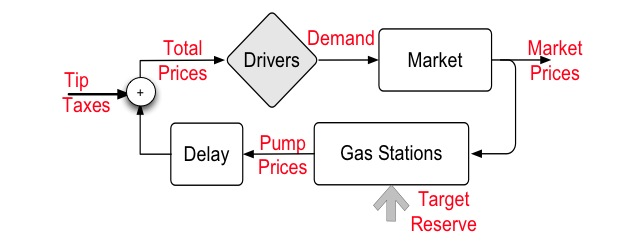
\includegraphics[width=4in]{gas-control-loop} 
   \caption{The gas control loop}
   \label{fig:gas-control-loop}
\end{figure}


This kind of block diagram is typical of many closed-loop (feedback) control systems where the system is said to reach {\em equilibrium} if the demand (for gas by drivers) matches the supply (of gas in the market). In data networks, users drive the demand on the network and have different utilities (expectations) when downloading music, playing games, making skype (voice/video) calls, or denying others service by launching a denial-of-service (DoS) attack! In turn, the network observes that user demand and sets ``prices", where the price could be real money, or it could be some measure (indication) of congestion (e.g., delay, loss), or it could represent additional resources that need to be allocated to avoid congestion. 

An important question is: {\em What is the goal of network design?} Is it to make users happy? You hope so! Then, mathematically, we say the goal of the network is to maximize the sum of utilities for all its users \cite{elastic:2006}.\footnote{We note that maximizing the sum of utilities involves interpersonal utility comparison, which needs to be ameliorated by linking to a common good, such as money.} Figure \ref{fig:net-control-loop} illustrates the data network equivalent of the gas control loop shown in Figure \ref{fig:gas-control-loop}. We next consider the modeling of user utility and network behavior (resource allocation), before introducing the optimization framework to study the (optimal) steady state for the users and network.


\begin{figure}[htbp] %  figure placement: here, top, bottom, or page
   \centering
   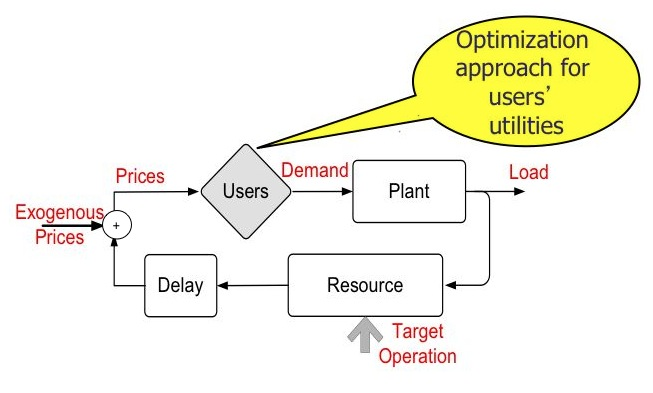
\includegraphics[width=4in]{net-control-loop.jpg} 
   \caption{The network control loop}
   \label{fig:net-control-loop}
\end{figure}


\subsection{Modeling the User}

Users typically have different utilities, i.e. different applications may perform differently based on the level of service (e.g., loss, delay) they get from the network. But, generally speaking, an application should perform better, the higher the rate (throughput) it is able to send at over the network. It is also generally the case that the gain (level of ``happiness") from higher throughput (i.e., {\em marginal utility}) diminishes as the throughput increases.  

Figure \ref{fig:concave-utility} shows such a utility function that is typical of what is called 
{\em elastic traffic} \cite{elastic:2006}. 
Formally, user $r$ has utility $U_r(x_r)$ when allocated rate $x_r > 0$. 
$U_r(x_r)$ is an increasing, strictly concave function of $x_r$ (see Figure \ref{fig:concave-function}).
And the derivative $\dot{U}_r(x_r) \rightarrow \infty$ as $x_r \rightarrow 0$,
and  $\dot{U}_r(x_r) \rightarrow 0$ as $x_r \rightarrow \infty$.
Throughout this chapter we assume strictly concave utilities.

\begin{figure}[htbp] %  figure placement: here, top, bottom, or page
   \centering
   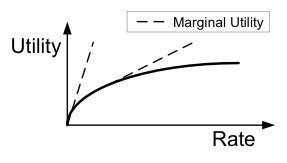
\includegraphics[width=2in]{concave-utility.jpg} 
   \caption{Concave utility function}
   \label{fig:concave-utility}
\end{figure}

\begin{figure}[htbp] %  figure placement: here, top, bottom, or page
   \centering
   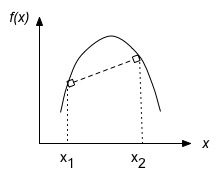
\includegraphics[width=2in]{concave-function.jpg} 
   \caption{Concave function. 
   A function $f(.)$ is said to be concave if $f(\alpha x_1 + (1-\alpha)x_2) \geq \alpha f(x_1) + (1-\alpha) f(x_2)$,
   i.e., for any two points $x_1$ and $x_2$, the straight line  that connects $f(x_1)$ and $f(x_2)$ is always below
   or equal to the function $f(.)$ itself. 
   Note that a differentiable concave function has a maximum value at some point $x_{max}$, and 
   that the derivative $\dot{f}(x_{max}) = 0.$
   A strictly concave function would have a strict inequality, whereas a convex function has a cup-like shape and
    has a minimum instead.}
   \label{fig:concave-function}
\end{figure}

\subsection{Modeling the Network}

We consider a network of $J$ resources, e.g., transmission links as they are typically considered the bottleneck. 
We denote by $R$ the set of all possible routes, and we assume that each user (source-destination traffic flow) is assigned to exactly one route $r$ (i.e., static single-path routing)\footnote{Given each user has one flow over a single path, we use the terms ``user", ``flow", and ``route" interchangeably.}.
We then define a 0-1 routing matrix $A$ such that:
$$
a_{jr} = \left\{ \begin{array}{rl} 
              1 & \mbox{ if resource $j$ is on route $r$} \\
              0 & \mbox{ otherwise}
              \end{array} \right.
$$
Figure \ref{fig:net-model} shows an example with three users  over a network of seven links: 
the first user (``blue" flow) uses the route made of links 1, 4, and 6;
the second user (``red" flow) uses the route made of links 2, 5, and 7;
and the third user (``green" flow) uses the route made of links 1, 4, and 7.
So the routing matrix has seven rows and three columns.

\begin{figure}[htbp] %  figure placement: here, top, bottom, or page
   \centering
   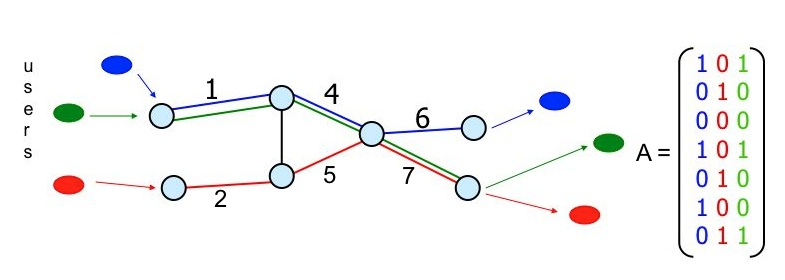
\includegraphics[width=5in]{net-model.jpg} 
   \caption{A network model}
   \label{fig:net-model}
\end{figure}


\subsection{The Optimization Problem}

Now we are ready to formulate a (centralized) optimization problem that allows the network to allocate rates to users so that the sum of their utilities is maximized \cite{Kelly-2001}. We refer to this problem as $SYSTEM(U, A, C)$ where the inputs are the user utility functions $U_r(.)$, the routing matrix $A$, and the (column) vector of link capacities $C$, and the output is the (column) vector of allocated rates $x$. \\

$SYSTEM(U, A, C):$
\begin{eqnarray*}
{\rm max} \sum_{r \in R} U_r(x_r) \ \\
{\rm subject~to}\ A x \leq C \ \\
{\rm over}\  x \geq 0
\end{eqnarray*}

For such an optimization problem, it is known that there exists a unique solution. This is the case because the function to optimize is strictly concave and the link capacity inequality constraints $A x \leq C$ form a so-called {\em convex set} (see Figure \ref{fig:convex-set}.)

\begin{figure}[htbp] %  figure placement: here, top, bottom, or page
   \centering
   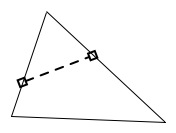
\includegraphics[width=1.5in]{convex-set.jpg} 
   \caption{A convex set. A convex set intuitively means that any linear combination of any two points located on the boundary of the region, which is formed by the linear inequalities, lies within the region itself. }
   \label{fig:convex-set}
\end{figure}

The practical challenge in solving this problem however is that the network does not know the utilities of its users, let alone its centralized nature makes it computationally expensive to solve!

To address these challenges, we start by decomposing the problem into $R$ problems, one for each user $r \in R$, and one problem for the network (we will later decompose this network problem further into individual resource problems). The network will present each user with a ``price" $\lambda_r$ (\$/bit).
Through these prices, the network attempts to infer user utilities.
Specifically, observing $\lambda_r$,
user $r$ will then choose an amount to pay $w_r$ (\$/second) for the service (that maximizes the user's utility), 
which in turn determines how much rate $x_r$ (bits/second) the user would get ($x_r = w_r/\lambda_r$).  
The network sets its prices $\lambda_r$ based on the load $x_r$, $\forall r$.

\subsection{Introducing Prices}

The decomposed optimization problem can then be stated in terms of the following user optimization problem, and network optimization problem. \\

$USER_r(U_r, \lambda_r):$
\begin{eqnarray*}
{\rm max}\ U_r(\frac{w_r}{\lambda_r}) \ \\
{\rm over}\ w_r \geq 0 
\end{eqnarray*}
where $\frac{w_r}{\lambda_r} = x_r $. Given the network price $\lambda_r$ and its own {\em private} utility function $U_r$, user $r$ determines how much it is willing to pay $w_r$ so as to maximize her own utility.

Knowing the vector $W=\{ w_r, \forall r \}$, its routing and capacity matrices, the network allocates user rates $x_r$ by optimizing some network function $f(x,W)$. Once $x_r$'s are obtained, 
prices are obtained as $\lambda_r = \frac{w_r}{x_r}$.\\

$NETWORK(A, C, W):$
\begin{eqnarray*}
{\rm max}\ \sum_{r \in R} f(x_r, w_r) \ \\
{\rm subject~to}\ A x \leq C \ \\
{\rm over}\ x \geq 0
\end{eqnarray*}

\subsection{Network Optimization}

The choice of the network function $f(x,W)$ determines how the capacity of the network gets allocated to users, and so how {\em fair} we might consider this allocation to be! For example, consider the following function:
\begin{eqnarray*}
f = \sum_{r \in R} w_r\; x_r
%\label{eq:greedy-net}
\end{eqnarray*}

Maximizing this function results in maximizing the total weighted throughput for all users. As a special case, for unit weights, the network optimization problem maximizes the total throughput through the network. This might seem to fly in the face of what we think is fair! Consider the following simple example (see Figure~\ref{fig:greedy-alloc}):
\begin{figure}[htbp] %  figure placement: here, top, bottom, or page
   \centering
   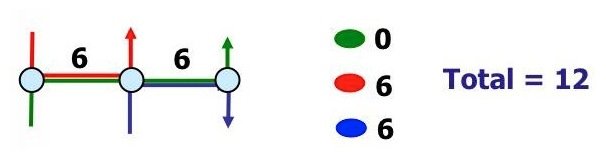
\includegraphics[width=4in]{greedy-alloc.jpg} 
   \caption{Greedy network allocation}
   \label{fig:greedy-alloc}
\end{figure}
given both links have capacities of 6 units, the total throughput allocated to all users is the total network capacity of 12 units. This can be achieved by allocating 6 units of capacity to each of the 1-link flows (users): the ``red" user and the ``blue" user, leaving the 2-link (``green") flow with no capacity allocated to its user. That does not seem ``fair"! A different function $f$ would allocate rates to users differently and so it would provide a different notion of fairness.

But, the big question is: {\em how do (should) we define fairness?} The research literature introduces many notions of fairness, most notably the so-called {\em max-min fairness}.

\subsubsection{Max-min Fairness}

Intuitively, max-min fairness means that  resources (link capacities) are allocated to users (flows) so that
the allocation is: 
\begin{enumerate}
\item {\em fair:} all users get equal share of a link, as long as users have demand that would fully consume their share, and
\item {\em efficient:} each link is utilized to the maximum load possible.
\end{enumerate}
In other words, if a user cannot consume its equal share of a link, then the excess capacity must be (recursively) allocated equally among high-demanding users. So, the final outcome is that low-demanding users get exactly what they need, while high-demanding users get equal allocations. Consider the following multi-link network example 
(see Figure~\ref{fig:max-min-alloc}):
\begin{figure}[htbp] %  figure placement: here, top, bottom, or page
   \centering
   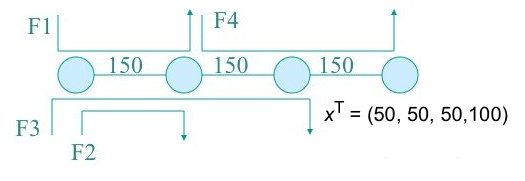
\includegraphics[width=4in]{max-min-fair.jpg} 
   \caption{Max-min fair capacity allocation}
   \label{fig:max-min-alloc}
\end{figure}
all links have capacities of 150 units and we assume elastic traffic sources, i.e., sources that would consume all what they can get. We start with the first (left-most) link since it is used by most users so it is the most loaded one. Each flow using that link gets allocated an equal share of $150/3=50$ units. Proceeding to the next loaded link, the middle one, each of its two flows should get an equal share of 75, however flow $F_3$ is limited by its first link to 50 units of throughput. Thus, flow $F_4$ gets the left-over from $F_3$ to a total allocation of $75+25=100$. The right-most link, at capacity of 150, does not limit the throughput  of $F_4$, which ends up using only 100 units of that link, leaving 50 unused. At the end of this process, we say that the max-min fair allocation  vector is $x^{\rm T} =(50,\; 50,\; 50,\; 100)$.

Mathematically, max-min fairness is achieved when the network maximizes the following function:
\begin{eqnarray*}
f = {\rm min}_{r \in R} \ x_r
%\label{eq:prop-fair}
\end{eqnarray*}
Intuitively, maximizing the minimum of allocated rates results in equalizing these rates, as long as users have enough demand that will consume these rates over the network.

\subsubsection{Proportional Fairness}

Another equally popular fairness definition is the so-called {\em (weighted) proportional fairness}. This notion of fairness is achieved when the network maximizes the following function:
\begin{eqnarray*}
f = \sum_{r \in R} w_r \; \lg(x_r)
\label{eq:prop-fair}
\end{eqnarray*}
Note that the log function is a concave, and strictly increasing function. Thus, given optimal rate allocation solution $x^*$, that is feasible, i.e.,\ $x^* \geq 0$ and $A\ x^* \leq C$, any other feasible solution $x$ will cause the aggregate proportional change $\sum_{r \in R} w_r \frac{x_r - x^*_r}{x^*_r}$ to be less than or equal zero.  To show this, for simplicity, assume one user and unit weight, so $f(x) = \lg(x)$. Expanding $f(x)$ into its first-order (linear) Taylor's approximation around $x^*$, we obtain:
\begin{eqnarray*}
f(x) \approx f(x^*) + (x - x^*) \dot{f}(x^*)
\end{eqnarray*}
Given the derivative $\dot{f}(x^*) = \frac{1}{x^*}$, we have:
\begin{eqnarray*}
f(x) \approx f(x^*) + \frac{(x - x^*)}{x^*} 
\end{eqnarray*}
Since $f$ is maximized at $x^*$, $f(x^*) \ge f(x)$ and so the proportional fairness condition must hold: 
\begin{eqnarray*}
\frac{x - x^*}{x^*} \leq 0 
\end{eqnarray*}
Note that the presence of weight $w_r$ intuitively means that user (flow) $r$ is equivalent to $w_r$ users with unit weight each.

\subsubsection{General Parameterized Utility}

If the network function $f(x)$ is a function of the utilities of its users $U(x)$, then the network is in fact maximizing a function of user utilities. Assuming each user $r$ has unit weight $w_r$, $U_r(x_r)$ can be generalized as \cite{Mo:2000}:
\begin{eqnarray*}
U_r(x_r) = \frac{x_r^{1-\alpha}}{1-\alpha}
\end{eqnarray*}
where $\alpha$ is a parameter that determines the fairness criterion of the network. More specifically, if $\alpha \rightarrow 0$, then a user's utility is linear in its allocated rate and the network is effectively maximizing the sum of user utilities $\sum_{r \in R} U_r(x_r) = \sum_{r \in R} x_r$, which in turn yields a greedy allocation that maximizes the total throughput over the network.

On the other hand, if $\alpha \rightarrow 1$, then this is equivalent to a log utility, yielding proportional fair allocation. To see this, let's take the derivative of $U_r(x_r)$:
\begin{eqnarray*}
\dot{U}_r(x_r) = \frac{(1-\alpha) x_r^{-\alpha}}{1-\alpha} \rightarrow \frac{1}{x_r}  \ {\rm as}\  \alpha \rightarrow 1
\end{eqnarray*}
By integrating $\dot{U}_r(x_r)$, we get back $U_r(x_r) = \lg(x_r)$.

Similarly, it can be shown that $\alpha \rightarrow \infty$ corresponds to a minimum utility, yielding a max-min fair allocation.

\subsection{Solution to Optimization Problem}
\label{sec:sol-opt}

Consider the case where the network is maximizing the weighted sum of the log of user rates, i.e., the network is trying to solve the following optimization problem that would yield a weighted proportional fairness allocation: \\

$NETWORK(A, C, W):$
\begin{eqnarray*}
{\rm max}\ \sum_{r \in R} w_r \; \lg(x_r) \\
{\rm subject~to}\ A x \leq C \ \\
{\rm over}\ x \geq 0
\end{eqnarray*}

We can solve this problem using the theory of constrained convex optimization using the Lagrangian technique. Specifically, we move the constraints into the objective function that we want to optimize, thus making the optimization problem effectively unconstrained. We do so by introducing so-called ``Lagrangian multipliers" into the new objective (Lagrangian) function $L$:
\begin{eqnarray*}
{\rm max}\ L = \sum_{r \in R} w_r \; \lg(x_r) + \lambda^T(C - Ax)\\
\end{eqnarray*}
The (row) vector $\lambda^T$ is a Lagrangian vector with a variable $\lambda_j$ for each link $j$ in the network.
Note that $L$ is a strictly concave function, thus a solution exists at which the derivatives of $L$ with respect to each $x_r$ and each $\lambda_j$ are equal to zero:
\begin{eqnarray}
  \frac{\partial L}{\partial x_r} & =   & \frac{w_r}{x_r} - \sum_{j \in r} \lambda_j
  \label{eqn:kkt1}
\end{eqnarray}
\begin{eqnarray}
  \frac{\partial L}{\partial \lambda_j} & =  & (C_j - \sum_{r \in j} x_r)  
  \label{eqn:kkt2}
\end{eqnarray}
The notation $j \in r$ indicates all links $j$ used by user (flow/route) $r$,
whereas $r \in j$ denotes all flows $r$ using link $j$, i.e. the total load on link $j$.

By equating the first set of equations (\ref{eqn:kkt1}) to zero, we obtain the (weighted proportionally fair) solution:
\begin{eqnarray}
x_r = \frac{w_r}{\sum_{j \in r} \lambda_j} 
\label{eqn:opt-x}
\end{eqnarray}
We obtain $\lambda_j$ by also equating the second set of equations (\ref{eqn:kkt2}) to zero. 
Note that $\lambda_j$ and $(C_j - \sum_{r \in j} x_r)$ must be greater than or equal to zero since negative values do not maximize the objective function $L$!  Furthermore, 
$(C_j - \sum_{r \in j} x_r) \geq 0$ ensures that the link capacity constraints $\sum_{r \in j} x_r \leq C_j$ are automatically satisfied. 
If $(C_j - \sum_{r \in j} x_r) = 0$ then $\lambda_j$ can be greater than zero. On the other hand,
if  $\lambda_j = 0$, then the associated link may not be fully utilized, i.e.\ $\sum_{r \in j} x_r < C_j$. 
Intuitively, $\lambda_j$ represents the ``cost" associated with link $j$, so it is zero if the link is under-utilized,
and positive if the link is allocated to capacity.

\paragraph{Example:}
Consider the example in Figure~\ref{fig:greedy-alloc} but now assume the network's objective of proportionally allocating its capacity, i.e., 
\begin{eqnarray*}
{\rm max}\  f = \lg(x_0) + \lg(x_1) + \lg(x_2) 
\end{eqnarray*}
subject to:
\begin{eqnarray*}
x_0 + x_1 \leq 6 \\
x_0 + x_2 \leq 6 \\
x_0, x_1, x_2 \geq 0
\end{eqnarray*}
where $x_0$, $x_1$, and $x_2$ are the rates allocated to the two-link flow (user), the first-link flow, and the second-link flow, respectively. \footnote{Note that since the objective (log) function is strictly increasing, then the $x_i$'s should be as large as possible to consume the total capacity of the links, so the two inequalities on link capacities could be turned into equalities. }

Using the Lagrangian's solution method, we obtain:
\begin{eqnarray*}
{\rm max}\ L = \lg(x_0) + \lg(x_1) + \lg(x_2) + \lambda_1(6- (x_0+x_1)) + \lambda_2(6- (x_0+x_2))
\end{eqnarray*}
Taking derivatives, we obtain:
\[
\begin{array}{ccc}
  \frac{\partial L}{\partial x_0} & =   & \frac{1}{x_0} - (\lambda_1+ \lambda_2)   \\ \\
  \frac{\partial L}{\partial x_1} & =   & \frac{1}{x_1} - \lambda_1   \\ \\
  \frac{\partial L}{\partial x_2} & =   & \frac{1}{x_2} - \lambda_2   \\ \\
  \frac{\partial L}{\partial \lambda_1} & =  & 6 -   (x_0+x_1)\\ \\
  \frac{\partial L}{\partial \lambda_2} & =  & 6 -   (x_0+x_2) \\
\end{array}
\]
Equating these derivatives to zero, the last two equations show full utilization of the link capacities and that $x_1=x_2$, while the first three equations give the following values of $x_i$'s: 
\begin{eqnarray*}
x_1 = x_2 = \frac{1}{\lambda_1} = \frac{1}{\lambda_2} = \frac{1}{\lambda} \\ \\
x_0 = \frac{1}{2 \lambda}
\end{eqnarray*}
Substituting in the capacity equations, we obtain the price of each link $\lambda$:
\begin{eqnarray*}
\frac{1}{2\lambda} + \frac{1}{\lambda} = 6 \\ 
\end{eqnarray*}
Thus, $\lambda = \frac{1}{4}$, and so $x_0 = 2$, and $x_1 = x_2 = 4$. 
Note that in this optimal case, each link is fully utilized to capacity, and the flow that traverses two links is charged twice for each link it traverses and so it gets allocated a lower rate.\footnote{As we will later see,
this proportional rate allocation is what TCP Vegas \cite{vegas:1995} provides.}
{\bf End Example.}\\


If the utility of each user $r$ is a log function in its allocated rate $x_r$, then the (weighted proportionally fair) network solution 
$x_r = \frac{w_r}{\sum_{j \in r} \lambda_j}$ is in fact, a solution to the whole system optimization problem that includes the network, as well as all users possibly trying to independently (in a distributed way) maximize their own log utilities.
However, in a distributed setting,
as noted earlier, even if the network knows the user utility functions,
the network allocates user rates based on their willingness to pay, $w_r$, which might be unknown to the network.
This lack of knowledge can be overcome by observing the demand behavior of the user $x_r$ and 
the price $\lambda_r = \sum_{j \in r} \lambda_j$, and so $w_r$ is computed as $w_r = x_r \; \lambda_r$.
Otherwise, the network can just assign some weights $w_r$ to users based on some preference policy.

The moral of the story is that in practice,
there is no central network controller that knows $W$ and can then allocate rates to users.
Each user and each resource (link) might have its own individual controller that will operate
independently and so we need to study the collective behavior of such composite system
and answer questions such as:
Would the system converge (stabilize) to a solution in the long term (i.e., reaching steady state)?
If so, 
is this solution unique and how far is it from the target (optimal) operating point?
In general, if the system gets perturbed, is it stable, i.e.
does it converge back to steady state,
and how long does it take to converge and how smooth or rough was that?
In control-theoretic terminology,
we refer to the response to such perturbation until steady state is reached
as the {\em transient response} of the system.
We refer to how far the system is from being unstable,
or the magnitude of perturbation that renders the system unstable, as
{\em stability margin}.

To formally address these questions, we will resort to the modeling of user and network dynamic behaviors,
in the form of differential (or difference) equations, then use well-known control-theoretic techniques
to study the overall transient and steady-state behavior of the system.

\section{The Control Problem}
\label{sec:control}

The basic control problem is to control the output of a system given a certain input.
For example, we want to control the user demand (sending rate) given the observed network price (e.g., packet loss or delay).
Similarly, we want to control the price advertised by a network resource given the demand (rates) of its users.

There is basically two kinds of control: open-loop control, and closed-loop (feedback) control.
In open-loop control systems, there is no feedback about the state of the system and the output of the system is controlled directly by the input signal. This type of control is thus simple, but not as common as closed-loop control.
An example of open-loop control system is a microwave that heats food for the input (specified) duration.

Feedback (closed-loop) control is more interesting and multiple controllers may be present in the same control loop. See Figure~\ref{fig:net-control-loop} where a user controller is present to control demand based on price, and a resource controller is also present to control price based on demand. Feedback control makes it possible to control the system well even if we can't observe or know everything, or if we make errors in our estimation (modeling) of the current state of the system, or if things change. This is because we can continually measure and correct (adapt) to what we observe (i.e., feedback signal). For example, in a congestion control system, we do not need to {\em exactly} know the number of users, the arrival rate of connections, or the service rate of the bottleneck resource, since each user would adapt its demand based on its own observed (measured, fed back) price, which reflects the current overall congestion of the bottleneck resource.

Associated with feedback control is a delay to observe the feedback (measured) signal, which is referred to as {\em feedback delay}. More precisely, feedback delay refers to the time taken from the generation of a control signal (e.g., updated user demand) until the process/system reacts to it (e.g., demand is routed over the network), this reaction takes effect at each resource (e.g., load is observed on each link), and this effect is fed back to the controller (e.g., price is observed by the user).

\subsection{System Models}

Models of controlled systems can be classified along four dimensions:
\begin{itemize}
\item {\em Deterministic versus stochastic models.} The latter models capture stochastic effects like noise and uncertainties.

\item {\em Time-invariant versus time-varying models.} The latter models contain system parameters that change over time.

\item {\em Continuous-time versus discrete-time models.} In the latter models, time is divided into discrete-time steps.

\item {\em Linear versus non-linear models.} The latter models contain non-linear dynamics.
 
\end{itemize}
In most of our treatment, we consider the simplest kind of models that are deterministic, time-invariant, continuous-time, and linear. In modeling a controlled system, we characterize the relationships among system variables as a function of time, i.e., dynamic equations. See Figure~\ref{fig:system-model} where functions $f$ and $h$ are generally non-linear functions. 
The function $f$ models the evolution of the state of the system $x$ as 
a function of the current state and system's input $u$.
The function $h$ yields system's output $y$ as a function of the current state and input values.
As we will see later, for mathematical tractability, we often linearize dynamic non-linear models or 
we only consider operation in a linear regime, for example, we ignore non-linearity when 
the buffer goes empty or hits full capacity.
\begin{figure}[htbp]
   \centering
   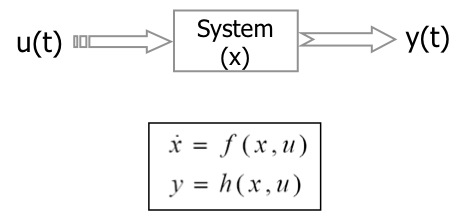
\includegraphics[width=3in]{system-model.jpg} % requires the graphicx package
   \caption{Typical system model}
   \label{fig:system-model}
\end{figure}

\subsection{Modeling Source and Network Dynamics}

Consider a source $r$ with log utility, i.e. $U_r(t) = w_r \; \lg(x_r)$, and 
a network that allocates rates in a weighted proportional fashion.
We saw earlier (cf.\ Section~\ref{sec:sol-opt}) that in steady state, the (optimal) solution (Equation \ref{eqn:opt-x}) is:
\begin{eqnarray}
x_r = \frac{w_r}{\lambda_r}
\label{eqn:kkt}
\end{eqnarray}
This can be re-written as $w_r - x_r \lambda_r = 0$.
Also, we saw that the optimal solution ensures that each link $l$ is fully utilized,
i.e. the load (total input rate) on link $l$, denoted by $y_l = \sum_{s: l \in s} x_s$, equals the link capacity $c_l$.

The dynamics of the sources and links can then be modeled such that these steady-state user rates and link loads are achieved. Specifically, we can write the dynamic (time-dependent) source algorithm as:
\begin{eqnarray}
\dot{x}_r (t) = k [w_r - x_r(t) \lambda_r(t)]
\label{eqn:source-adapt}
\end{eqnarray}
where $k$ is a proportionality factor.
Note that $w_r$ represents how much user $r$ is willing to pay,
whereas $x_r(t) \lambda_r(t)$ represents the cost (price) of sending at that rate.
Intuitively, the user sending rate increases (decreases) when the difference between these two quantities is positive (negative). And in steady state, $\dot{x}_r(\infty) \rightarrow 0$, and so we obtain the steady-state solution  $x_r = \frac{w_r}{\lambda_r}$ (as expected).

Given that the derivative of  $U_r(t)$, $\dot{U}_r(t) = \frac{w_r}{x_r}$, 
the source rate adaptation algorithm can be re-written as:
\begin{eqnarray*}
\dot{x}_r (t) = k x_r(t) [\dot{U}_r(t) - \lambda_r(t)]
\end{eqnarray*}
%
\begin{eqnarray}
\dot{x}_r (t) = K(t) [\dot{U}_r(t) - \lambda_r(t)]
\label{eqn:source-alg}
\end{eqnarray}
Intuitively, the user increases its sending rate if the marginal utility (satisfaction) is higher than the price that the user will pay, otherwise the user decreases its sending rate.


We can also write a dynamic equation for the adaptation in the link price $\lambda^l(t)$, called the link pricing algorithm:
\begin{eqnarray}
\dot{\lambda}^l(t) = h (y_l(t) - c_l)
\label{eqn:link-alg}
\end{eqnarray}
where $h$ is a proportionality factor, and the total price, $\lambda_r(t)$, for user $r$,
is the sum of the link prices along the user's route, i.e. $\lambda_r(t) =  \sum_{l: l \in r} \lambda^l(t)$.
Intuitively, the link price increases if the link is over-utilized (i.e. $y_l(t) > c_l$), otherwise
the link price decreases.
Note that at steady state, $\dot{\lambda}^l(\infty) \rightarrow 0$, and 
we obtain the steady-state optimal solution $y_l = c_l$ (as expected).

It turns out that the source and link algorithms, Equations \ref{eqn:source-alg} and \ref{eqn:link-alg},
represent general user and resource adaptation algorithms that collectively determine 
the transient and steady behavior of the whole system.
In what follows, we use the form of Equation \ref{eqn:source-alg} to reserve engineer different versions
of TCP and deduce the utility function that the TCP source tries to maximize.


\subsection{TCP and RED}
 
Many analytical studies considered the network system composed of TCP sources over a network of queues that employ a certain queue management policy. Examples of TCP variants include Reno, SACK \cite{Fall:1996}, NewReno, Vegas \cite{vegas:1995}, FAST \cite{fast:2006}, etc. Examples of queue management policies include Drop Tail, RED \cite{red:1993}, REM \cite{REM:2001}, PI \cite{PI:2000}, etc. One of the most widely studied instantiation is that of TCP sources over a RED bottleneck queue --- see Figure~\ref{fig:TCP-RED-diagram}.
We start by modeling the dynamic behavior of a TCP source, i.e., 
the time-dependent relationship between its transmission window (or sending rate) and 
its observed loss rate or delay (price).
We do so for both TCP Reno and Vegas versions, and also deduce their utilities.
Then, we model the buffering process inside the network (more precisely, the bottleneck queue),
assuming a linear regime (i.e., ignoring non-linearities due to the buffer becoming empty or full).
Using the average buffer length, we model the dynamic behavior of RED and how 
it generates packet losses (or markings) as indication of congestion (price).
This overall model represents the closed-loop feedback system shown in 
the block diagram of Figure~\ref{fig:TCP-RED-diagram}, 
which can then be analyzed using control-theoretic techniques.
\begin{figure}[htbp]
   \centering
   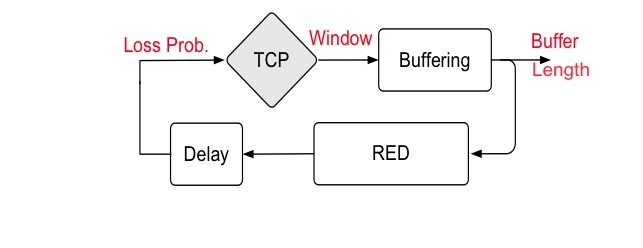
\includegraphics[width=4in]{tcp-red.jpg} % requires the graphicx package
   \caption{TCP Reno over RED feedback control system}
   \label{fig:TCP-RED-diagram}
\end{figure}

\paragraph{Modeling TCP Reno:} First, consider the modeling of TCP Reno, where the congestion window {\em cwnd} is increased by $1/cwnd$ for every acknowledged TCP segment / non-loss, i.e., it is (roughly) increased by 1 every round-trip time, and {\em cwnd} is decreased by half for every loss. Thus, we can write the following equation for changes in the congestion window of a single TCP flow, where $p$ is the segment loss probability:

\begin{eqnarray*}
\Delta cwnd = \frac{1}{cwnd} (1-p) - \frac{cwnd}{2} p
\end{eqnarray*}
Let $x$ denote the sending rate, and $T$ the round-trip time, thus $x = \frac{cwnd}{T}$.
Assuming acknowledgments (ACKs) come equally spaced, 
the time between ACKs (or lack thereof) is given by $\frac{T}{cwnd}$.
Thus, we can re-write the above equation in terms of change in {\em rate} as:
\begin{eqnarray*}
\frac{d}{dt}  cwnd(t) = \frac{\frac{1}{cwnd(t)} (1-p(t)) - \frac{cwnd(t)}{2} p(t)}{\frac{T}{cwnd(t)}}
\end{eqnarray*}
Dividing both sides by $T$, we get:
\begin{eqnarray*}
\frac{d}{dt} x(t) = \frac{\frac{1}{x(t) T^2} (1-p(t)) - \frac{x(t)}{2} p(t)}{\frac{1}{x(t)}}
\end{eqnarray*}


\begin{eqnarray}
\frac{d}{dt} x(t) = \frac{1}{T^2} (1-p(t)) - \frac{{x(t)}^2}{2} p(t)
\label{eqn:reno}
\end{eqnarray}

%\begin{eqnarray}
%\frac{d}{dt} x(t) = \frac{1}{T^2}  - (\frac{1}{T^2} + \frac{{x(t)}^2}{2}) p(t)
%\label{eqn:reno}
%\end{eqnarray}

Let's denote the loss probability $p(t)$ of TCP connection $r$ as $p_r(t)$.
$p_r(t)$ depends on the current load on path $r$,
and can be approximated by the sum of loss probabilities experienced on individual links $j \in r$ 
along the connection's path.
More specifically,
\begin{eqnarray*}
p_r(t) = \sum_{j \in r} p_j(\sum_{s: j \in s} x_s(t))
\end{eqnarray*}


Assuming small $p$ such that $(1-p) \approx 1$, we can re-write Equation~\ref{eqn:reno} as follows:
\begin{eqnarray*}
\frac{d}{dt} x(t) = \frac{1}{T^2}  - \frac{{x(t)}^2}{2} p(t)
\end{eqnarray*}

\begin{eqnarray}
\frac{d}{dt} x(t) = \frac{{x(t)}^2}{2} [\frac{2}{T^2 x(t)^2}  - p(t)]
\label{eqn:reno-util}
\end{eqnarray}

Comparing Equation \ref{eqn:reno-util} with Equation \ref{eqn:source-alg},
we can deduce the utility function of a TCP Reno source:
\begin{eqnarray*}
\dot{U}(x) = \frac{2}{T^2 x^2} 
\end{eqnarray*}
Integrating $\dot{U}(x)$ we get:
\begin{eqnarray*}
U(x) =  \frac{-2}{T^2 x} 
\end{eqnarray*}
Observe that maximizing Reno's utility results in minimizing the quantity $\frac{1}{x}$, which can be viewed as the ``potential delay" as it is inversely proportional to the allocated rate $x$. 
Thus, a network allocation based on such utility is referred to as {\em minimum potential delay fair allocation}.

\paragraph*{Example:} 
Revisting the example in Figure~\ref{fig:greedy-alloc} but now assume the network's objective is to allocate its capacity according to the minimum potential delay fair allocation, i.e., 
\begin{eqnarray*}
{\rm max} \ f = \frac{-1}{x_0} + \frac{-1}{x_1} + \frac{-1}{x_2} 
\end{eqnarray*}
subject to:
\begin{eqnarray*}
x_0 + x_1 \leq 6 \\
x_0 + x_2 \leq 6 \\
x_0, x_1, x_2 \geq 0
\end{eqnarray*}
where $x_0$, $x_1$, and $x_2$ are the rates allocated to the two-link flow (user), the first-link flow, and the second-link flow, respectively. 

Using the Lagrangian's solution method, we obtain:
\begin{eqnarray*}
{\rm max}\ L =  \frac{-1}{x_0} + \frac{-1}{x_1} + \frac{-1}{x_2} + \lambda_1(6- (x_0+x_1)) + \lambda_2(6- (x_0+x_2))
\end{eqnarray*}
Taking derivatives, we obtain:
\[
\begin{array}{ccc}
  \frac{\partial L}{\partial x_0} & =   & \frac{1}{x_0^2} - (\lambda_1+ \lambda_2)   \\ \\
  \frac{\partial L}{\partial x_1} & =   & \frac{1}{x_1^2} - \lambda_1   \\ \\
  \frac{\partial L}{\partial x_2} & =   & \frac{1}{x_2^2} - \lambda_2   \\ \\
  \frac{\partial L}{\partial \lambda_1} & =  & 6 -   (x_0+x_1)\\ \\
  \frac{\partial L}{\partial \lambda_2} & =  & 6 -   (x_0+x_2) \\
\end{array}
\]
Equating these derivatives to zero, the last two equations show full utilization of the link capacities and that $x_1=x_2$, while the first three equations give the following values of $x_i$'s: 
\begin{eqnarray*}
x_1 = x_2 = \frac{1}{\sqrt{\lambda_1}} = \frac{1}{\sqrt{\lambda_2}} = \frac{1}{\sqrt{\lambda}} \\ \\
x_0 = \frac{1}{\sqrt{2 \lambda}}
\end{eqnarray*}
Substituting in the capacity equations, we obtain the price of each link $\lambda = 0.08$,
and so $x_0 \approx 2.5$, and $x_1 = x_2 \approx 3.5 $. 

Note that in this optimal case, each link is fully utilized to capacity, and 
the rate allocated to a flow is inversely proportional to the square-root of the price it observes along its path.

Note also that this captures the well-known {\em steady-state} relationship between the throughput of a TCP Reno source and the inverse of the square-root of the {\em loss probability} observed by the TCP source \cite{tcp-thru:2000}.
A TCP Reno source adapting based on Equation \ref{eqn:reno} would converge to such steady-state throughput value.
{\bf End Example.}\\


\paragraph{Modeling TCP Vegas:} 
Now, let us consider the modeling of another version of TCP --- TCP Vegas \cite{vegas:1995}.
This version, unlike Reno, tries to {\em avoid} congestion, rather than induce loss and 
and then adapt the transmission (congestion) window to it.  
The basic idea behind Vegas is to calculate the {\em actual} throughput of the connection
as $\frac{w(t)}{T(t)}$, where $w(t)$ is the current window size,
and $T(t)$ is the measured round-trip time (RTT) over the connection's path.
This RTT includes queueing delay, as well as propagation delay $D$.
Ideally, with no congestion, the ideal throughput can be computed by the source
as $\frac{w(t)}{D}$, where $D$ is estimated using the minimum RTT recently observed by the source.
To ensure high utilization of the network, we want some queueing, i.e. 
the actual throughput is lower than the ideal one, but not too low to start causing congestion (i.e. buffer overflow
at the bottleneck link resulting in losses).
Vegas then adapts $w(t)$ based on some target difference, $\alpha$, 
between the actual throughput and the ideal one.
More specifically,
the window increases if $(\frac{w(t)}{D} - \frac{w(t)}{T(t)}) < \alpha$,
decreases if $(\frac{w(t)}{D} - \frac{w(t)}{T(t)}) > \alpha$,
and stays the same otherwise. This dynamic source behavior,
i.e. change in window over time, can be modeled as:
\begin{eqnarray*}
\frac{dw(t)}{dt} = k [\alpha - (\frac{w(t)}{D} - \frac{w(t)}{T(t)})]
\end{eqnarray*}
This can be re-written as:
\begin{eqnarray*}
\frac{dw(t)}{dt} = \frac{k}{D} [\alpha D - (w(t) - \frac{w(t)}{T(t)}D)]
\end{eqnarray*}
Denoting the sending rate (throughput) by $x(t) = \frac{w(t)}{T(t)}$, 
and $\gamma = \frac{k}{D}$, we have:
\begin{eqnarray*}
\frac{dw(t)}{dt} = \gamma [\alpha D - (w(t) - x(t)D)]
\end{eqnarray*}
At steady state, as $\dot{w}(\infty) \rightarrow 0$, we have:
\begin{eqnarray*}
w - x D = \alpha D
\end{eqnarray*}
Observe that the left-hand side represents the difference between the window size of packets
injected by the source, and the number of packets in flight / propagating along the path (represented by
the product of throughput and propagation delay). Thus,
the left-hand side represents the number of packets in the bottleneck queue,
and $\alpha D$ denotes the {\em target} queue occupancy of the bottleneck link.
Intuitively, Vegas tries to maintain a small number of $\alpha D$ packets
(i.e., 1-2 packets)
in the bottleneck queue to maintain both small delay and high (100\%) utilization.
Section~\ref{sec:linear} uses control theory to analyze a Vegas-like transmission model.

Given that $x = w/T$, we get:
\begin{eqnarray*}
x T - x D = \alpha D
\end{eqnarray*}
Denoting the queueing delay by $Q$, we have $T = Q + D$, and so: 
\begin{eqnarray*}
x Q = \alpha D
\end{eqnarray*}
\begin{eqnarray*}
x = \frac{\alpha D}{Q}
\end{eqnarray*}
Comparing with Equation \ref{eqn:kkt}, we can deduce that
the willingness to pay $w_r$ for a Vegas user $r$ is $\alpha D$
and that the price $\lambda_r$ experienced by the user is the queueing delay $Q$.

Now, to deduce the utility function that a Vegas user tries to maximize,
let us write its rate adaptation equation following Equation \ref{eqn:source-adapt}:
\begin{eqnarray*}
\dot{x}_r(t) = k [\alpha D - x_r(t) Q(t)]
\end{eqnarray*}
\begin{eqnarray*}
\dot{x}_r(t) = K(t) [\frac{\alpha D}{x_r(t)} - Q(t)]
\end{eqnarray*}
Thus, comparing with Equation \ref{eqn:source-alg}, we deduce:
\begin{eqnarray*}
\dot{U}_r(t) = \frac{\alpha D}{x_r(t)} 
\end{eqnarray*}
Integrating, we obtain:
\begin{eqnarray*}
U_r(t) = \alpha D \; \lg(x_r(t)) 
\end{eqnarray*}
Recall that maximizing such user utilities results in a weighted proportional fair allocation.

\paragraph{Modeling RED:}
Let us now consider the modeling of the buffer and associated RED queue management algorithm \cite{red:1993}.
Figure~\ref{fig:red} shows how RED tries to avoid congestion by dropping (or marking) packets with probability $p_c$ 
as a (non-linear) function of the average queue length $v$.
\begin{figure}[htbp]
   \centering
   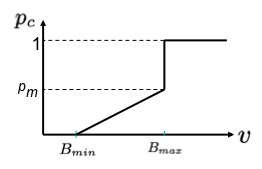
\includegraphics[width=2in]{red.jpg} % requires the graphicx package
   \caption{RED dropping (or marking) function}
   \label{fig:red}
\end{figure}
First, we model the evolution of the queue length $b(t)$ as 
a function of the total input rate, $y(t) = \sum x_s(t)$, and (bottleneck) link capacity, $C$:
\begin{eqnarray*}
\dot{b}(t) =  y(t) - C
\end{eqnarray*}
Denoting by $v(t)$, the Exponential Weighted Moving Average (EWMA) of the queue length:
\begin{eqnarray*}
v(t+\delta) = (1 - \alpha) v(t) + \alpha b(t)
\end{eqnarray*}
\begin{eqnarray*}
v(t+\delta) - v(t) = \alpha (b(t) - v(t))
\end{eqnarray*}
Given $v(t)$ gets updated at the link rate, i.e. $\delta = \frac{1}{C}$,
and $\dot{v}(t) \approx \frac{v(t+\delta) - v(t)}{\delta}$, we have:
\begin{eqnarray*}
\dot{v}(t) = \alpha C \; (b(t) - v(t))
\end{eqnarray*}
This last equation represents the dynamic model of RED averaging, which in turn determines the price $p_c(t)$ that users experience. 

To simplify the model and gain insight, let us ignore the (hard) non-linearities of the RED function
and consider only the linear region:
\begin{eqnarray*}
p_c(t) = \sigma v(t) + \eta = \sigma \int \dot{v}(t) dt + \eta = \sigma \int \alpha C(b(t) - v(t)) dt + \eta
\end{eqnarray*}
where $\sigma = p_m/(B_{max}-B_{min})$, and $\eta= -p_m\;B_{min}/(B_{max}-B_{min})$.

To gain more insight, let us further ignore the RED averaging, 
assuming that the price is set in proportion to the actual queue length,
$B_{min}=0$ and $p_m = 1$, then we have:
\begin{eqnarray*}
p_c(t) = \frac{1}{B_{max}} \; b(t)
\end{eqnarray*}
Differentiating both sides, we obtain:
\begin{eqnarray*}
\dot{p}_c(t) = h \; \dot{b}(t) = h(y(t) - C)
\end{eqnarray*}
where $h = \frac{1}{B_{max}}$.
Comparing with Equation \ref{eqn:link-alg}, 
the packet dropping (congestion marking) probability, $p_c(t)$,
represents the ``price", i.e. Lagrangian multiplier, observed by users of this buffer.
Note that at steady state, $\dot{p}_c(\infty) \rightarrow 0$,
and so $y=C$, i.e. the link is fully utilized at steady state.

\subsection{Solving the Feedback Control System}

We have developed dynamic (time-dependent) models for users (sources), e.g. TCP, and the network (links), e.g. RED,
and the interaction between them through prices.
The next step is to solve for the transient and steady-state performance of such system.
Solving such systems is challenging because of inherent non-linearilities,
e.g. the ``hard" non-linearities (discontinuities) in the RED pricing function,
or the ``soft" non-linearity of TCP where the sending rate changes quadratically in the current rate.
Non-linear control theory becomes a useful tool as it deals directly with non-linear differential equations.
Specifically, a method called {\em Lyapunov} \cite{Ogata:2010} allows one to study convergence (stability) by showing that the value of some positive function of the state  of the system continuously decreases as the system evolves over time.
Finding such a Lyapunov function can be challenging, and 
transient performance can often only be obtained by solving the system equations numerically.

To this end, a technique called {\em linearization} can prove more tractable
where the non-linear system is approximated by a set of {\em linear} equations around a single operating point (state).
See Figure \ref{fig:linearize}.
\begin{figure}[htbp]
   \centering
   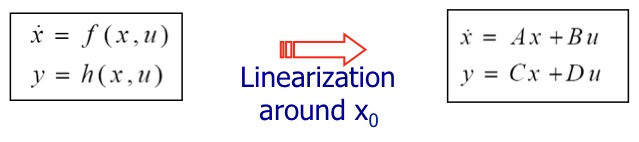
\includegraphics[width=3in]{linearize.jpg} % requires the graphicx package
   \caption{Linearization}
   \label{fig:linearize}
\end{figure}
With linearization, we become concerned with {\em local stability} and study perturbations around the operating point
using standard (linear) control theory. 
By local stability, we mean that if the system is perturbed within a small region around the operating point 
then the system will converge and stabilize back to that point.
This is in contrast to {\em global stability} where the original (non-linear) system is shown to 
converge from {\em any} starting state.
To linearize the non-linear system around an operating point,
the basic idea is to expand the non-linear differential equation into 
a Taylor series around that point and then ignore high-order terms.

In what follows, we briefly review some basics of classical control theory for linear systems,
then we introduce non-linear control theory. We also show examples of control theoretic analysis for 
the dynamic models introduced above.
For more detailed background on control theory,
we refer the reader to \cite{Ogata:2010,Keshav:2010,Lu:2001}.

\section{Linear Control Theory}  
\label{sec:linear}

In linear control theory, we transform differential equations in the {\em time domain} to algebraic equations in the so-called {\em frequency} or {\em Laplace} domains. Once this Laplace transformation is done, we use simple algebra to study the performance of the system without the need for going back to the (complicated) time domain. Specifically, we can transform a function $f(t)$ to an algebraic function $F(s)$, referred to as the Laplace transform of $f(t)$, as follows:
\begin{eqnarray*}
F(s) = \int_0^{\infty} f(t) e^{-st} dt
\end{eqnarray*}
where $s$ is a complex variable: $s = \sigma + j \omega$, $\sigma$ is the real part of $s$, denoted by $Re(s)$,
and $\omega$ is the imaginary part of $s$, denoted by $Im(s)$.

\paragraph{Example (Unit step function):}
The Laplace transform of a unit step function $u(t)$, where $u(t) = 1$ if $t > 0$, and $u(t) = 0$ otherwise, is given by:
\begin{eqnarray*}
U(s) = \int_0^{\infty} 1 . e^{-st} dt = \frac{1}{s}
\end{eqnarray*}


\paragraph{Example (Impulse function):}
The Laplace transform of a unit impulse function $\delta(t)$, where $\delta(t) = 1$ if $t = 0$, and $\delta(t) = 0$ otherwise, is given by:
\begin{eqnarray*}
U(s) = \int_0^{\infty} 1 . e^{-st} dt = e^{0} = 1
\end{eqnarray*}
 
Table~\ref{tab:transforms} lists basic Laplace transforms.
\begin{table}[htdp]
\caption{Basic Laplace transforms}
\begin{center}
\begin{tabular}{|c|l|} \hline
Impulse input:	$f(t) = \delta(t)$ & $F(s) = 1$ \\ [2ex]
Step input: 	$f(t) = a.1(t)$	& $F(s) = a/s$ \\[2ex]
Ramp input: 	$f(t) = a.t$		& $F(s) = a/s^2$ \\[2ex]
Exponential:	$f(t) = e^{at}$	& $F(s) = 1/(s-a)$ \\[2ex]
Sinusoid input:	$f(t) = \sn(at)$	& $F(s) = a/(s^2+a^2)$ \\ [2ex]\hline
\end{tabular}
\end{center}
\label{tab:transforms}
\end{table}%

Table~\ref{tab:composition} lists basic composition rules, 
where $\L[f(t)]$ denotes the Laplace transform of $f(t)$, i.e. $F(s)$.
\begin{table}[htdp]
\caption{Composition rules}
\begin{center}
\begin{tabular}{|c|} \hline 
Linearity:	$\L[a\ f(t) + b\ g(t)] = a F(s) + b G(s)$ \\[2ex]
Differentiation: $\L[df(t)/dt] =  sF(s) - f(0) = sF(s)$ if $f(0) = 0$ \\[2ex]
Integration: $\L[\int f(\tau) d\tau] = F(s)/s$ \\[2ex]
Convolution: $y(t) = g(t) \Conv u(t) = \int_0^{t} g(t-\tau) u(\tau) d \tau \Rightarrow Y(s) = G(s) U(s)$ \\ [2ex] \hline
\end{tabular}
\end{center}
\label{default}
\label{tab:composition} 
\end{table}%

\paragraph{Example:}
Consider the following second-order linear, time-invariant differential equation, where $y(t)$ represents the output of a system, and $u(t)$ represents the input:
\begin{eqnarray*}
a_2 \ddot{y}(t) + a_1 \dot{y}(t) + a_0 y(t) = b_1 \dot{u}(t) + b_0 u(t)
\end{eqnarray*}
In the time domain, if we represent the system by $g(t)$,
then $y(t)$ can be obtained by convolving $u(t)$ with $g(t)$, i.e. $y(t)=g(t) \Conv u(t)$.
This involves a complicated integration over the system responses,
$g(t-\tau)$, to impulse inputs of magnitude $u(\tau)$, for all $0 < \tau < t$.

Assuming $y(0)=u(0)=0$, taking the Laplace transform of both sides, we obtain:
\begin{eqnarray*}
a_2 s^2 Y(s) + a_1 s Y(s) + a_0 Y(s) = b_1 s U(s) + b_0 U(s)
\end{eqnarray*}
\begin{eqnarray*}
Y(s) = \frac{(b_1 s  + b_0)}{(a_2 s^2 + a_1 s  + a_0)}  U(s) = G(s) U(s)
\end{eqnarray*}
Thus, in the Laplace domain, the output $Y(s)$ can be obtained by simply multiplying 
$G(s)$, called the {\em transfer function} of the system, with $U(s)$.
We can then take the inverse Laplace transform, $\L^{-1}[Y(s)]$, to obtain $y(t)$,
or as we will later see, we can simply analyze the stability of the system by examining 
the roots of the denominator of the transfer function $G(s)$ and their location in the complex s-domain.

Note that because $Y(s) =  G(s)$ for an impulse input, i.e. $U(s)=1$,
the transfer function $G(s)$ is also called {\em impulse response function}.

\subsection{Modeling a Vegas-like System}

Consider the system in Figure~\ref{fig:vegas-control} where a controller $G_c$ is used to match
the queue length $b(t)$ to a target $B_r$ by controlling the input window or sending rate $x(t)$.
The output rate from the queue is denoted by $c(t)$.
\begin{figure}[htbp]
   \centering
   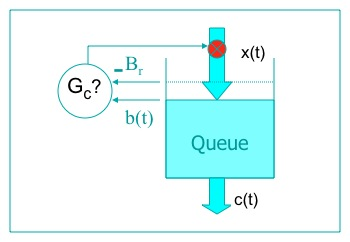
\includegraphics[width=2.5in]{vegas-control.jpg} % requires the graphicx package
   \caption{Vegas-like system}
   \label{fig:vegas-control}
\end{figure}
The goal is to first write down the differential equations that model the different components of the system,
then instead of solving the equations in the time domain, we will transform them to the Laplace domain and
analyze the stability of the system algebraically.

We start by describing the buffer evolution as:
\begin{eqnarray*}
\frac{d}{dt} b(t) = x(t) - c(t)
\end{eqnarray*}
Then, $x(t)$ is the output of convolving the error $e(t) = B_r - b(t)$ with the controller function $G_c(t)$,
 i.e. 
\begin{eqnarray*}
x(t) = G_c(t) \Conv e(t)
\end{eqnarray*}

Now, taking the Laplace transforms, we obtain:
\begin{eqnarray*}
s B(s) = X(s) - C(s)  \Rightarrow  B(s) = \frac{X(s) - C(s)}{s}
\end{eqnarray*}
\begin{eqnarray*}
X(s) = G_c(s) E(s) = G_c(s) (B_r(s) - B(s))
\end{eqnarray*}

Figure~\ref{fig:vegas-BD} shows the system using its transfer functions and their input/output flows,
where $G_0 = \frac{1}{s}$.
This is called the {\em block diagram} and provides a powerful pictorial tool.
\begin{figure}[htbp]
   \centering
   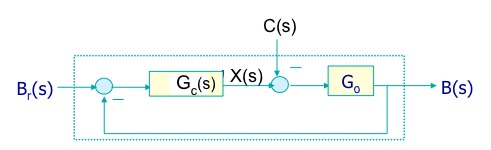
\includegraphics[width=4in]{vegas-BD.jpg} % requires the graphicx package
   \caption{Block diagram of Vegas-like system}
   \label{fig:vegas-BD}
\end{figure} 
From the block diagram, one can write the algebraic equation of the output in terms of the input(s).
Dropping the ``s" parameter for convenience:
\begin{eqnarray*}
\frac{(B_r - B) G_c - C}{s} = B
\end{eqnarray*}
Rearranging, we get:
\begin{eqnarray}
B = \frac{G_c}{s + G_c} B_r - \frac{1}{s + G_c} C
\label{eqn:vegas-TF}
\end{eqnarray}
Note that the system has two inputs: $B_r(s)$ and $C(s)$, subjected to two transfer functions,
$\frac{G_c(s)}{s + G_c(s)}$ and $\frac{-1}{s + G_c(s)}$, respectively, and 
adding their responses we obtain the output $B(s)$.

\subsection{Proportional Control and Stability of Vegas-like System}

One basic controller $G_c$ is referred to as {\em Proportional (P)} controller, where
the controlled variable $x(t)$ is simply set in proportion to the error signal,
i.e. $x(t) = K_p\ e(t)$.
In this case, $G_c(s)$ is simply the constant $K_p$. 

Substituting in Equation \ref{eqn:vegas-TF}, we have:
\begin{eqnarray}
B(s) = \frac{K_p}{s + K_p} B_r(s) - \frac{1}{s + K_p} C(s)
\label{eqn:P-ess}
\end{eqnarray}

An important question is: {\em does the P-controller make the system stable?}
More precisely, if we subject the system to impulse input(s),
does the system converge back to a quiescent state?
Control theory gives a systematic way to answer such stability question by
examining the roots of the denominator of the system's transfer function,
called the {\em characteristic equation}. 
In this case,
the characteristic equation is:
\begin{eqnarray*}
s + K_p = 0 \Rightarrow s = - K_p
\end{eqnarray*}
The system is stable if the roots (also called {\em poles}) lie in the left-hand side of the complex s-plane.
Thus this system is stable if $- K_p < 0 \Rightarrow K_p > 0$.

Note that we did not need to go back to the time domain to analyze the stability of the system.
But let's do that here to understand why poles on the  left-hand side of the s-plane makes the system stable.
Taking the inverse Laplace transform of  Equation \ref{eqn:P-ess}, and assuming impulse inputs,
i.e. $B_r(s) = C(s) = 1$, we get:
\begin{eqnarray*}
b(t) = K_p e^{-K_p t} - e^{-K_p t}
\end{eqnarray*}
We can then see that $b(t)$ decays exponentially over time, starting from $b(0)=(K_p-1)$.
We say that the system is stable or exhibits {\em overdamped response}.

We can also analyze transient performance by noting that
$b(0)=(K_p-1)$ represents an {\em overshoot} response to the impulse input,
and that this overshoot is lower for lower $K_p$.
See Figure~\ref{fig:overdamped}.
So by controlling $K_p$, referred to as the {\em controller gain},
we can also control the system's transient response.

\begin{figure}[htbp] %  figure placement: here, top, bottom, or page
   \centering
   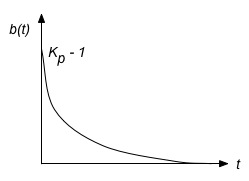
\includegraphics[width=1.6in]{overdamped.jpg} 
   \caption{Overdamped response}
   \label{fig:overdamped}
\end{figure}

\subsection{Proportional Integral Control and Stability of Vegas-like System}

Another type of controller is known as {\em Proportional Integral (PI)} controller where
the controlled variable $x(t)$ is set in proportion to the integral of the error signal,
i.e. $x(t) = K_i\ \int e(t) \; dt$.
In this case, 
taking the Laplace transform, $G_c(s) = \frac{K_i}{s}$. 
Note that the integration means that the history of the error is used to control $x(t)$.

Substituting in Equation \ref{eqn:vegas-TF}, we have:
\begin{eqnarray}
B(s) = \frac{K_i}{s^2 + K_i} B_r(s) - \frac{s}{s^2 + K_i} C(s)
\label{eqn:PI-ess}
\end{eqnarray}

To analyze stability, we again examine the poles of the characteristic equation:
\begin{eqnarray*}
s^2 + K_i = 0  \Rightarrow s = \stackrel{+}{-} j \sqrt{K_i}
\end{eqnarray*}
Given $K_i > 0$, the two imaginary conjugate poles lie in the left-hand side of the complex s-plane,
and so the system is stable, though {\em critically} stable as we explain next.

To convince ourselves, let us go back to the time domain by taking the inverse Laplace transform:
\begin{eqnarray*}
\L^{-1}[\frac{K_i}{s^2 + K_i}] = \L^{-1}[\frac{K_i}{(s - j \sqrt{K_i})(s + j \sqrt{K_i})}] =
\L^{-1}[\frac{A}{(s - j \sqrt{K_i})} + \frac{B}{(s + j \sqrt{K_i})}] 
\end{eqnarray*}
And for some values of $A$ and $B$, this yields:
\begin{eqnarray*}
A e^{j \sqrt{K_i}t} + B e^{- j \sqrt{K_i}t}
\end{eqnarray*}
Given the fact that $e^{j \theta} =  \cs \; \theta + j \ \sn \; \theta$,
the function in the time domain oscillates in a sinusoidal fashion.
Although the time function does not decay over time,
it does {\em not} diverge, i.e. it is not unstable! 
So, we consider such a system to have bounded oscillations in response to
impulse input and we say that it is {\em critically (or marginally) stable} or 
the system exhibits  {\em undamped oscillatory response}.
Note that a higher value of $K_i$ results in more oscillatory behavior.
See Figure~\ref{fig:undamped}.

\begin{figure}[htbp] %  figure placement: here, top, bottom, or page
   \centering
   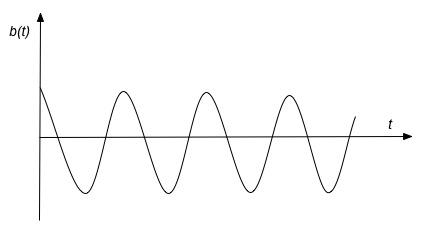
\includegraphics[width=2.5in]{undamped.jpg} 
   \caption{Undamped response}
   \label{fig:undamped}
\end{figure}

\subsection{Stability and Pole Placement}

More formally, a linear time-invariant system is stable if
all poles of its transfer function are in the left-hand side of the s-plane,
i.e. the real part of all poles is negative.
Figure \ref{fig:pole-loc} shows the time response given the location 
of the poles. 

Note that if the poles are complex conjugates and strictly in the left-hand side 
of the s-plane, the system is stable as oscillations in response to impulse input decay over time,
and we say that the system exhibits {\em underdamped response}.
\begin{figure}[htbp]
   \centering
   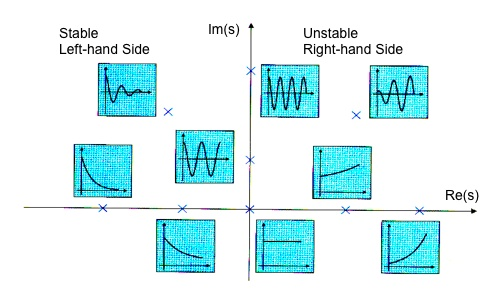
\includegraphics[width=4in]{pole-loc.jpg} % requires the graphicx package
   \caption{Time response depending on pole location}
   \label{fig:pole-loc}
\end{figure}

\subsection{Transient Performance and Steady-state Error}
\label{sec:transient}

Besides stability, there are other performance metrics of interest that
characterize the transient performance of the system and the quality 
of the steady state.
Figure \ref{fig:transient} shows several of these metrics,
including the time for the controlled variable to reach its peak (maximum) value,
the time to reach the target, 
the maximum overshoot over the steady-state value,
and the error that remains at steady state
when the system stabilizes away from the desired target value.

\begin{figure}[htbp]
   \centering
   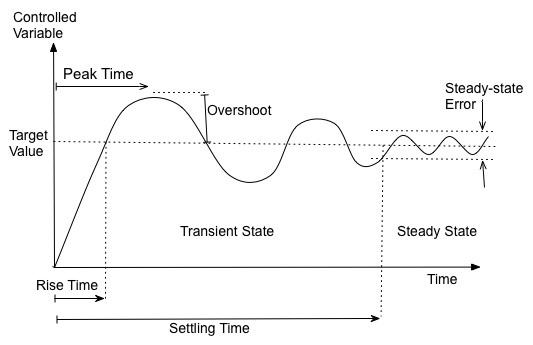
\includegraphics[width=4in]{perf-spec.jpg} % requires the graphicx package
   \caption{Performance Metrics}
   \label{fig:transient}
\end{figure}

For our Vegas-like system,
the controlled variable is the window size, i.e. number of packets
allowed into the system. The response is the queue length, which
we measure and compare to the target  buffer size.
A ``good" system is one that converges quickly to the desired target
with minimum oscillations (i.e., overshoots and undershoots) and
with almost zero steady-state error.


\subsection{Steady-state Error}

In control theory, the steady-state error of a stable system is defined as:
\begin{eqnarray*}
e_{ss} = \lm_{t \rightarrow \infty}\ e(t) = \lm_{t \rightarrow \infty}\  (r(t) - b(t))
\end{eqnarray*}
where $r(t)$ is the reference input, and $b(t)$ is the system output (response).
This error reflects how accurately the system can achieve the desired target,
which is chosen to be a step input.

We state without proof the Final Value Theorem \cite{Ogata:2010}:
\begin{eqnarray*}
e_{ss} = \lm_{t \rightarrow \infty}\ e(t) = \lm_{s \rightarrow 0}\ s\ E(s)
\end{eqnarray*}
This theorem allows us to calculate $e_{ss}$ algebraically in the Laplace domain.

\paragraph{Example (P-control of Vegas-like system):}
\begin{eqnarray*}
E(s) = B_r(s) - B(s)
\end{eqnarray*}
Substituting for $B(s)$ from Equation \ref{eqn:P-ess} and using the Final Value Theorem, we obtain:
\begin{eqnarray*}
e_{ss} = \lm_{s \rightarrow 0}\ s\ [B_r(s) - \frac{K_p}{s + K_p} B_r(s) + \frac{1}{s + K_p} C(s)]
\end{eqnarray*}

Assuming step inputs, i.e. $B_r(s) = \frac{B_r}{s}$ and $D(s) = \frac{D}{s}$, we have:
\begin{eqnarray*}
e_{ss} = \lm_{s \rightarrow 0}\ [B_r - \frac{K_p}{s + K_p} B_r + \frac{1}{s + K_p} C] = \frac{C}{K_p}
\end{eqnarray*}
Recall that under the P-controller, the system is (overdamped) stable, i.e. 
$b(t)$ approaches the target $B_r$ without oscillations, however,
at steady state, $b(t)$ misses the target by $\frac{C}{K_p}$ and 
stabilizes at a value lower than $B_r$.
Notice that the higher the service capacity $C$ is, the larger the steady-state error.
So, to decrease the steady-state error, the controller gain $K_p$ could be increased.
However, increasing $K_p$ increases the overshoot.
A tradeoff clearly exists between transient performance and steady-state performance,
and one has to choose $K_p$ to balance the two and meet desired operation goals.
 {\bf  End Example.}


\paragraph{Example (PI-control of Vegas-like system):}
\begin{eqnarray*}
E(s) = B_r(s) - B(s)
\end{eqnarray*}
Substituting for $B(s)$ from Equation \ref{eqn:PI-ess} and using the Final Value Theorem, we obtain:
\begin{eqnarray*}
e_{ss} = \lm_{s \rightarrow 0}\ s\ [B_r(s) - \frac{K_i}{s^2 + K_i} B_r(s) + \frac{s}{s^2 + K_i} C(s)]
\end{eqnarray*}

Assuming step inputs, i.e. $B_r(s) = \frac{B_r}{s}$ and $C(s) = \frac{C}{s}$, we have:
\begin{eqnarray*}
e_{ss} = \lm_{s \rightarrow 0}\ [B_r - \frac{K_i}{s^2 + K_i} B_r + \frac{s}{s^2 + K_i} C] = 0
\end{eqnarray*}
Although the steady-state error is zero under the PI-controller, 
recall that the system is critically stable, i.e. it converges to the target while
oscillating. Decreasing the controller gain $K_i$ decreases these oscillations,
however at the expense of longer time to reach steady state.
This illustrates again the inherent tradeoff between transient performance
and the quality of the steady state.


\section{Analyzing the Stability of Non-linear Systems}
\label{sec:nonlinear}

As we have seen, linear control theory can be applied to non-linear systems if we assume
a small range of operation around which the system behavior is linear
or approximately linear. This linear analysis
is simple to use, and the system, if stable, has a unique equilibrium point. 

On the other hand, most control systems are non-linear, and operate over a wide range of
parameters, and multiple equilibrium points may exist. In this case, non-linear control theory 
could be more complex to use.

In what follows, we first consider a non-linear model of the adaptation of sources and network,
and use a non-linear control-theoretic stability analysis method, 
called {\em Lyapunov method} \cite{Ogata:2010}.
Then, we linearize the system and illustrate the application of linear control-theoretic analysis.

\subsection{Solving Non-linear Differential Equations}

Recall Vegas-like source adaptations from Equation \ref{eqn:source-adapt}:
\begin{eqnarray*}
\frac{d x_r(t)}{dt} = k [w_r - x_r(t) p_r(t)]
\end{eqnarray*}
where $p_r(t)$ represents the total price observed by user $r$ along its path.
Note that this differential equation is non-linear since $p_r(t)$ is a function of the rates $x_s(t)$:
\begin{eqnarray*}
p_r(t) = \sum_{{\rm link}\; l \in {\rm route}\; r}\ p_l(t) = \sum_{l \in r}\ p_l(\sum_{s: l \in s} x_s(t))
\end{eqnarray*}
We assume that the pricing function $p_l(y)$ is monotonically increasing in the load $y$.

At steady state, if the system stabilizes, setting the derivatives to 0, we obtain the steady-state solution:
\begin{eqnarray*}
 k [w_r - x_r\; p_r] = 0 \Rightarrow x_r = \frac{w_r}{p_r} = \frac{w_r}{\sum_{l \in r}\; p_l}
\end{eqnarray*}

To prove stability, we use the non-linear method of Lyapunov.
The basic idea is to find a positive scalar function $V(x(t))$, we call the Lyapunov function,
and show that the function monotonically increases (or decreases)
over time, approaching the steady-state solution.

Define $V(x)$ as follows:
\begin{eqnarray*}
V(x) = \sum_{r \in R} w_r \; \lg(x_r) - \sum_{j \in J} \int_{0}^{\sum_{s: j \in s} x_s} p_j(y) dy
\end{eqnarray*}
Finding a suitable Lyapunov function that shows stability is tricky and more of an art!
If you can't find one, it does {\em not} mean that the system is not stable.
Note that this $V(x)$ has some special meaning:
the first term represents the utility gain from making users happy,
while the second term represents the cost in terms of price.
So $V(x)$ represents the net gain.
Also, note that since the first term is concave because of the log function,
and the second term is assumed to be monotonically increasing,
then the resulting $V(x)$ is concave, i.e. it has a maximum value.

To show that $V(x(t))$ is strictly convergent, we want to show that $\frac{dV(x(t))}{dt} > 0$,
which implies that $V(x(t))$ strictly increases (i.e. the net gain keeps increasing over time), 
until the system stabilizes and reaches steady state when $\frac{dV(x(t))}{dt} = 0$ 
(i.e. the net gain $V(x)$ reaches its maximum value).

First, we note:
\begin{eqnarray*}
\frac{\partial V(x)}{\partial x_r} = \frac{w_r}{x_r} - \sum_{j \in r} p_j(\sum_{s: j \in s} x_s)
\end{eqnarray*}

Then:
\begin{eqnarray*}
\frac{V(x(t))}{dt} = \sum_{r \in R} \frac{\partial V(x(t))}{\partial x_r} \; \frac{d x_r(t)}{dt}
\end{eqnarray*}

\begin{eqnarray*}
\frac{V(x(t))}{dt} = \sum_{r \in R} [\frac{w_r}{x_r} - \sum_{j \in r} p_j(\sum_{s: j \in s} x_s(t))] \; k [w_r - x_r(t) p_r(t)]
\end{eqnarray*}

\begin{eqnarray*}
\frac{V(x(t))}{dt} = \sum_{r \in R} k \;x_r(t) [\frac{w_r}{x_r} - \sum_{j \in r} p_j(\sum_{s: j \in s} x_s(t))]^2 > 0
\end{eqnarray*}

Observe that this non-linear stability analysis shows that the system is stable, no matter what 
the initial state $x(0)$ is. This property is referred to as {\em global stability},
which is in contract to {\em local stability} that we prove when the system is linearized locally
around a certain operating point as we will see next.  

\subsection{Linearizing and Solving Linear Differential Equations}

As noted earlier, finding Lyapunov functions to prove global stability of non-linear control systems,
even for simple models, is challenging. For example, consider more sophisticated models
with feedback delay, different regions of TCP operation (e.g., timeouts, slow-start),
queue management with different operating regions (e.g., RED), and
challenging or adversarial environments (e.g., exogenous losses over wireless links or due to DoS attacks).

Using linearization, we can separately study simpler linear models around the different points (regions)
of operation. More specifically, we linearize the system around a single operating point $x^*$ and
study perturbations around $x^*$, i.e. if we perturb the system away from $x^*$ to a point $x(0)$ such that the initial perturbation $\delta x(0) = x(0) - x^*$, we want to show that $\delta x(t)$ diminishes over time and the system returns to its original state $x^*$, i.e. $\delta x(t) \rightarrow 0$. In this case, we say that the system is {\em locally stable} around $x^*$.

Let's consider again the Vegas-like source adaptation and assume, for simplicity, a single user over a single resource:
\begin{eqnarray*}
\frac{d x(t)}{dt} = k [w - x(t) p(x(t))]
\end{eqnarray*}

Define the perturbation $\delta x(t) = x(t) - x^*$. Then we can write:
\begin{eqnarray*}
\frac{d (\delta x(t) + x^*)}{dt} = k [w - (\delta x(t) + x^*) p((\delta x(t) + x^*))]
\end{eqnarray*}

Expanding the non-linear term $p((\delta x(t) + x^*))$ into its first-order Taylor series:
\begin{eqnarray*}
p((\delta x(t) + x^*)) \approx p(x^*) + \dot{p}(x^*) \delta x(t)
\end{eqnarray*}

Substituting with this linear approximation, we get:
\begin{eqnarray*}
\frac{d \delta x(t)}{dt} = k [w - (\delta x(t) + x^*) \{p(x^*) + \dot{p}(x^*) \delta x(t)\}]
\end{eqnarray*}

\begin{eqnarray*}
\frac{d \delta x(t)}{dt} = k [w - \delta x(t) p(x^*) - x^* p(x^*) - \dot{p}(x^*) \delta^2 x(t) - \dot{p}(x^*) x^* \delta x(t)]
\end{eqnarray*}

If $x^*$ is the optimal steady-state point, we know that $w - x^* p(x^*) = 0$ (cf.\ Equation~\ref{eqn:kkt}). 
Also, given small perturbation $\delta x(t)$, $\delta^2 x(t) \approx 0$.
Then, we have:
\begin{eqnarray*}
\frac{d \delta x(t)}{dt} = k [ - \delta x(t) p(x^*)  - \dot{p}(x^*) x^* \delta x(t)]
\end{eqnarray*}

\begin{eqnarray*}
\frac{d \delta x(t)}{dt} = -k [p(x^*)  + x^* \dot{p}(x^*) ]\; \delta x(t)
\end{eqnarray*}

Let $k[p(x^*)  + x^* \dot{p}(x^*)] = \gamma$, we have:
\begin{eqnarray}
\frac{d \delta x(t)}{dt} = - \gamma\ \delta x(t)
\label{eqn:linearized}
\end{eqnarray}

This is now a linear differential equation, which unlike the original non-linear differential equation,
we can easily study using linear control-theoretic techniques, or
in this simple case, solve by straightforward integration:
\begin{eqnarray*}
\int_{0}^{t} \frac{d\; \delta x(t)}{\delta x(t)} = - \gamma\ \int_{0}^{t} dt
\end{eqnarray*}

\begin{eqnarray*}
\lg (\delta x(t)) -  \lg (\delta x(0)) = - \gamma t
\end{eqnarray*}

\begin{eqnarray*}
\lg (\frac{\delta x(t)}{\delta x(0)})  = - \gamma t  
\end{eqnarray*}

\begin{eqnarray*}
\delta x(t)  = \delta x(0)\; e^{- \gamma t}
\end{eqnarray*}

Note that from this time-domain analysis, the system is shown to be stable, i.e. the perturbation vanishes over time and the system returns to its original state $x^*$. We also observe that the system response decays exponentially from its original perturbation $\delta x(0)$, i.e. without oscillations, and so the response is classified as {\em overdamped}.

If the linearized differential equation modeling the system were more complicated, it is much easier to transform it into the Laplace domain and analyze the system algebraically. 
Denoting $\delta x(t)$ by $u(t)$, the Laplace transform of $\delta x(t)$ by $U(s)$, and taking the Laplace transform of Equation \ref{eqn:linearized}, we get:
\begin{eqnarray*}
s\; U(s) - u(0) = - \gamma\ U(s)
\end{eqnarray*}

\begin{eqnarray*}
U(s)  = \frac{u(0)}{s + \gamma }  
\end{eqnarray*}

For stability analysis, we examine the location of the poles (roots) of the characteristic equation $s + \gamma = 0$, yielding the pole $s = -\gamma$. Since the pole is strictly in the left-side of the s-plane, given $\gamma > 0$, the system is stable and its response is overdamped.

To evaluate the steady-state error, we define the error as $e(t) = u(0) - u(t)$, and applying the Final Value Theorem with an impulse perturbation of magnitude $u(0)$, i.e. $U(0)=u(0)$, we obtain:
\begin{eqnarray*}
e_{ss} = \lm_{s \rightarrow 0}\ s E(s) = \lm_{s \rightarrow 0}\ s [u(0) - \frac{u(0)}{s + \gamma } ] = 0
\end{eqnarray*}
So, there is no steady-state error.

\subsubsection{Effect of Feedback Delay and Nyquist Stability Criterion}

As we just noted above, the power of solving the linearized model in the Laplace domain comes when the model is even slightly more complicated. For example, let us consider a feedback delay $T$ such that Equation \ref{eqn:linearized} looks like:
\begin{eqnarray*}
\frac{d u(t)}{dt} = - \gamma\ u(t - T)
\end{eqnarray*}

Taking the Laplace transform, and noting that the Laplace transform of a delayed signal $u(t-T)$ is
$e^{-sT} U(s)$, we obtain:
\begin{eqnarray*}
s U(s) - u(0) = - \gamma\ e^{-sT} U(s)
\end{eqnarray*}

\begin{eqnarray*}
U(s) = \frac{u(0)}{s + \gamma\ e^{-sT}}
\end{eqnarray*}

Then, the characteristic equation is:
\begin{eqnarray}
s + \gamma\ e^{-sT} = 0
\label{eqn:delayed}
\end{eqnarray}
which we need to solve to locate the poles and determine the stability of the system. 

To solve such characteristic equation, we resort to another control-theoretic method called the {\em Nyquist stability criterion} \cite{Ogata:2010}.  To this end, we introduce, without proof,
the {\em Cauchy's principle} \cite{Ogata:2010}, 
which states that given $F(s)$, and we plot $F(s)$ as we vary $s$ along a certain contour (trajectory) in the s-plane --- see Figure~\ref{fig:cauchy} --- and denote the following:
\begin{itemize}
\item $Z$: the number of {\em zeros} of $F(s)$, i.e. the roots of the numerator of $F(s)$, inside the contour.

\item $P$: the number of {\em poles} of $F(s)$, i.e. the roots of the denominator of $F(s)$, inside the contour.

\item $N$: the number of times that the plot of $F(s)$ encircles the origin in the $F(s)$-plane, 
such that an encirclement is negative if it is in the opposite direction of the s-contour.\footnote{
The example in Figure~\ref{fig:cauchy} shows that $N=-3$.
The value of $N$ is negative because the s-contour that is mapped to $F(s)$ is clockwise,
whereas the resulting $F(s)$ plot is counter-clockwise.
Moreover, the $F(s)$ path encircles the origin in the  $F(s)$-plane three times --
drawing a line emanating from  the origin intersects the $F(s)$ path three times.
}
\end{itemize}

Then the following relationship holds:
\begin{eqnarray*}
Z = P + N
\end{eqnarray*}

\begin{figure}[htbp]
   \centering
   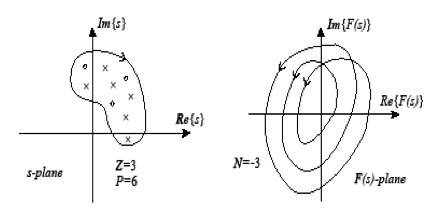
\includegraphics[width=4in]{cauchy.jpg} % requires the graphicx package
   \caption{Cauchy's principle}
   \label{fig:cauchy}
\end{figure}

The Nyquist method applies the Cauchy's principle as follows.
Let's say we want to analyze the stability of a closed-loop control system
whose forward transfer function is $G(s)$ and its feedback transfer function is $H(s)$---see Figure \ref{fig:closed-loop}.
Then, the closed-loop transfer function is given by $\frac{G(s)}{1+G(s) H(s)}$,
where $G(s)H(s)$ is referred to as the {\em open-loop} transfer function.
The characteristic equation is given by: $F(s) = 1 + G(s) H(s) = 0$.
Observe that the zeros of $F(s)$ are the closed-loop poles,
and the poles of $F(s)$ are the poles of $G(s)H(s)$ (so-called ``open-loop" poles).
\begin{figure}[htbp]
   \centering
   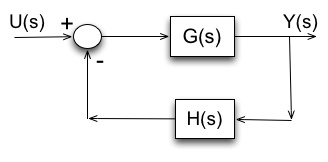
\includegraphics[width=3in]{closed-loop.jpg} % requires the graphicx package
   \caption{Typical closed-loop control system}
   \label{fig:closed-loop}
\end{figure}

By taking the s-contour to be around the right-side (i.e. unstable side) of the s-plane
(see Figure \ref{fig:s-contour}),
and noting the number of {\em unstable} open-loop poles $P$
and the number of encirclements $N$ around the origin in the $F(s)$-plane, we determine 
the number of {\em unstable} zeros $Z$ of $F(s)$, i.e. number of unstable closed-loop poles,
using Cauchy's relationship: $Z = P + N$.
If $P = 0$ and $N = 0$, then $Z = 0$ implies that there are no {\em unstable} closed-loop poles
and so the closed-loop system is stable.\footnote{
Note that a pole on the imaginary axis is not considered unstable and
the s-contour avoids such a pole and we show it as a small circle around it.
}
\begin{figure}[htbp]
   \centering
   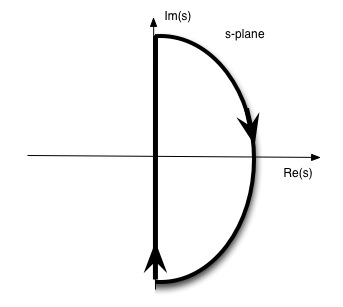
\includegraphics[width=3in]{s-contour.jpg} % requires the graphicx package
   \caption{Contour around the unstable right-side of the s-plane}
   \label{fig:s-contour}
\end{figure}

This process can be slightly simplified if instead of plotting $F(s)$,
we instead plot the open-loop transfer function: $G(s)H(s)$ and 
observe its encirclements of the $(-1, j 0)$ point in the $G(s)H(s)$-plane,
instead of  the origin $(0, j 0)$ in the $F(s)$-plane.
Given there are no poles of $G(s)H(s)$ in the right-side of the s-plane, i.e. $P=0$,
in order for the closed-loop system to be stable,
the plot of  $G(s)H(s)$ should not encircle -1 as we vary $s$ along the contour enclosing
the right-side of the s-plane.
We are mostly interested in varying $s$ along the imaginary axis,
i.e. $s = j \omega$ where $\omega$ varies from 0 to $\infty$.
This is because the plot for $\omega$ from $- \infty$ to 0 is symmetric,
and the plot for the semi-circle as $s \rightarrow \infty$ maps to the origin in the $G(s)H(s)$-plane.
Thus, we are interested in plotting $G(j \omega) H(j \omega)$
as $\omega$ varies from 0 to $\infty$.

\paragraph{Example:}
Let's go back to the characteristic equation in Equation \ref{eqn:delayed}:
\begin{eqnarray*}
s + \gamma\ e^{-sT} = 0  \Rightarrow F(s) = 1 + \frac{\gamma}{s} e^{-sT} \Rightarrow G(s)H(s) = \frac{\gamma}{s} e^{-sT}
\end{eqnarray*}
Note that $G(s)H(s)$ does not have any unstable poles, i.e. $P=0$. 
In particular, $s=0$ is considered a (critically) stable pole.

Ignoring the constant factor $\gamma$ for now, we want to plot:
\begin{eqnarray*}
\frac{e^{-j \omega T}}{j \omega} \ \ \ \ \ \  \omega: 0 \rightarrow \infty
\end{eqnarray*}

Noting that $e^{j \theta} = \cs \; \theta + j\; \sn \; \theta$, we have:
\begin{eqnarray*}
e^{-j \omega T} = \cs(\omega T) - j\; \sn(\omega T) 
\end{eqnarray*}
Then,
\begin{eqnarray*}
\frac{e^{-j \omega T}}{j \omega} = - j \frac{\cs(\omega T)}{\omega} - \frac{\sn(\omega T)}{\omega} 
\end{eqnarray*}

Since we are interested in determining intercepts with the real-axis of $G(j \omega) H(j \omega)$
and whether they occur to the right or left of -1 (see Figure~\ref{fig:ex-nyquist}),
we want to determine the values of $\omega$ 
for which the imaginary part of $G(j \omega) H(j \omega)$, i.e. $- \frac{\cs(\omega T)}{\omega}$, is zero.
Such intercepts occur when $\omega T = \frac{\pi}{2}, \frac{3 \pi}{2}, \cdots$, when the cosine value is zero.

\begin{figure}[htbp] %  figure placement: here, top, bottom, or page
   \centering
   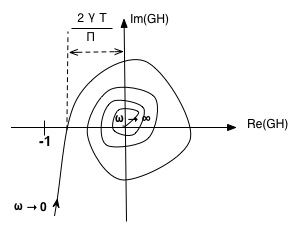
\includegraphics[width=3in]{ex-nyquist.jpg} 
   \caption{Example showing the effect of feedback delay}
   \label{fig:ex-nyquist}
\end{figure}

Now, at these values of $\omega T$, we can determine the points of interception along the real-axis, i.e.
the magnitude $|G(j \omega) H(j \omega)|$ when the plot intercepts the real-axis:
\begin{eqnarray*}
 - \frac{\sn(\omega T)}{\omega} = - \frac{1}{\frac{\pi}{2T}}, +\frac{1}{\frac{3 \pi}{2T}}, \cdots
\end{eqnarray*}
For the system to be stable, $|G(j \omega) H(j \omega)|$ at these intercepts must be less than 1,
so the $G(s) H(s)$ plot does not encircle -1.
This is the case if after restoring the constant factor $\gamma$ we initially ignored, 
the following condition holds:
\begin{eqnarray*}
\gamma \frac{2T}{\pi} < 1
\end{eqnarray*}  {\bf End Example.}


Observe that $T$ is the feedback delay, so as $T$ gets larger, it becomes harder to satisfy the stability condition.
Intuitively, this makes sense since a larger feedback delay results in outdated feedback (measurements) and 
it becomes impossible to stabilize the system. 
This is the fundamental reason why TCP over long-delay paths does not work, and
architecturally, control has to be broken up into smaller control loops.


\section{Routing Dynamics}
\label{sec:routing}

So far, we assumed routes taken by flows to be static. In general, routes may also be adapted based on feedback on link prices (reflecting load, delay, etc.), 
albeit over a longer timescale of minutes, hours or even days compared to that of milliseconds for sending rate adaptation.
Figure \ref{fig:block-routing} shows a block diagram that includes both route and sending rate adaptation.
\begin{figure}[htbp]
   \centering
   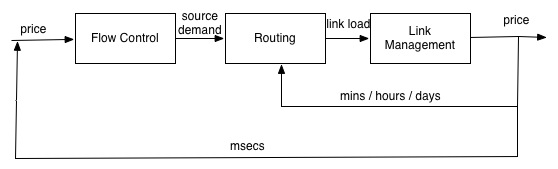
\includegraphics[width=5in]{block-routing.jpg} % requires the graphicx package
   \caption{Block diagram with both flow and routing control}
   \label{fig:block-routing}
\end{figure}

Figure \ref{fig:routing-conv} illustrates the general process of adaptation.
Flow or routing control determines the amount of load directed to a particular link based
on the link's observed price --- 
relative to that of other possible links on alternate routes in the case of routing.
We call this mapping from link price $\lambda$ to link load $x$, 
the {\em response function} $G(\lambda)$.
Given link load, a certain price is observed for the link.
We call such load-to-price mapping, the {\em pricing (feedback) function} $H(x)$.
The process of adaptation is then an iterative process:
\begin{eqnarray*}
\lambda = H(x) \\
x = G(\lambda)
\end{eqnarray*}

\begin{figure}[htbp]
   \centering
   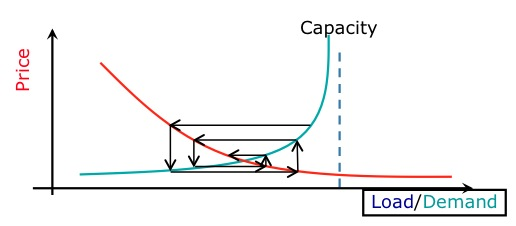
\includegraphics[width=4in]{routing-conv.jpg} % requires the graphicx package
   \caption{Convergence}
   \label{fig:routing-conv}
\end{figure}


We can then write:
\begin{eqnarray*}
\lambda = H(G(\lambda))  = F(\lambda)
\end{eqnarray*}
where $F(\lambda)$ is an {\em iterative} function whose stable (fixed) point $\lambda^*$ is the intersection of
the response function and the pricing function.
Figure \ref{fig:contractive} illustrates convergence to a fixed point.
Starting from an initial $\lambda_0$,
we find $F(\lambda_0)$,
then projecting on the $45^{o}$ line we obtain $\lambda_1 = F(\lambda_0)$,
which we use to find $F(\lambda_1)$,
and this iterative process continues until we reach the fixed point.

\begin{figure}[htbp]
   \centering
   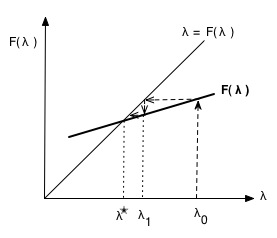
\includegraphics[width=3in]{contractive.jpg} % requires the graphicx package
   \caption{Contractive mapping}
   \label{fig:contractive}
\end{figure}


In order to converge to that fixed point, $F(\lambda)$ must be a so-called {\em contractive mapping}.
Intuitively,
$F(\lambda)$ is contractive iff its slope is less than 1, i.e.
$|F(\lambda_2) - F(\lambda_1)| < \alpha |\lambda_2 - \lambda_1|$, $\alpha < 1$.
Figure \ref{fig:non-contractive} illustrates a mapping that results in divergence.

\begin{figure}[htbp]
   \centering
   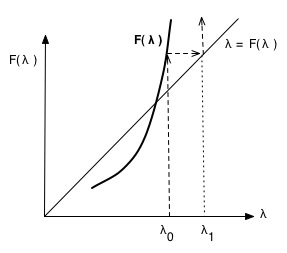
\includegraphics[width=3in]{non-contractive.jpg} % requires the graphicx package
   \caption{Divergent mapping}
   \label{fig:non-contractive}
\end{figure}

Intuitively, the use of Lyapunov functions to prove convergence tests whether the iterative process
describing the evolution of the system over time is a contractive mapping, i.e. 
the distance to the fixed point keeps shrinking at every iteration.

\paragraph{Example:}
Consider the adaptive routing of $N > 0$ unit-rate flows over two possible paths whose prices are given by
{\em monotonically increasing} functions
$p_1(x)$ and $p_2(N-x)$, where $x$ represents the number of flows (or load) routed on the first path.
Note that $x$ completely defines the state of the system.
Also, assume that routing to the least-loaded path is done gradually, to avoid wild oscillations,
where $0 < \alpha < 1$ of the flows are re-routed.
Using a discrete-time model where routes are adapted at discrete-time steps, 
we can write the following difference equations:
$$
x(t+1) = \left\{ \begin{array}{rl} 
               x(t) + \alpha \; [N - x(t)]  & \mbox{if  $p_1(x(t)) \leq p_2(N -  x(t))$ } \\
               x(t) - \alpha \; x(t) & \mbox{otherwise}
                        \end{array} \right.
$$

At steady state, this system might converge to one of two possible stable (fixed) points.
One possibility is obtained when substituting with $x(t) \rightarrow x^*$ in the first difference equation: 
$x(t) \rightarrow x^* \Rightarrow x^* = x^* + \alpha [N - x^*] \Rightarrow x^* = N$, 
so all traffic will end up getting routed on the first path. 
A {\em necessary} condition to reach that $x^* = N$ fixed point is that $p_1(N) \leq p_2(0)$, i.e. 
the first path is least loaded (priced) even when all $N$ flows are on it.

Another possibility is obtained when substituting with $x(t) \rightarrow x^*$ in the second difference equation:
$x(t) \rightarrow x^* \Rightarrow x^* = x^* - \alpha x^* \Rightarrow x^* = 0$, 
so all traffic will end up getting routed on the second path. 
A {\em necessary} condition to reach that $x^* = 0$ fixed point is that $p_1(0) > p_2(N)$, i.e. 
the second path is least loaded (priced) even when all $N$ flows are on it.

We can show convergence to one of these fixed points depending on which necessary condition holds: 
$p_1(N) \leq p_2(0)$ or $p_1(0) > p_2(N)$.

Let's assume $p_1(N) \leq p_2(0)$ holds. We want to define a Lyapunov function $V(x) \geq 0$ and show that
$V(x(t+1)) \leq V(x(t))$ for some or all starting state $x(0)$, 
i.e. $V(x)$ monotonically decreases toward the $x^* = N$ fixed point
where equality holds.
If there are only certain values of the starting state $x(0)$ for which the system converges then
such conditions must hold, in addition to the necessary condition,
for convergence to happen. 
In this case, we say that the necessary condition by itself is not sufficient for convergence.

Define $V(x) = N - x$. Note that $V(x) \geq 0$ because $0 \leq x \leq N$, and $V(x) = 0$ when $x = N$, i.e. at the fixed point. 
So, under convergence, we expect $V(x)$ to monotonically decrease toward zero. 
Substituting for $x(t+1)$ in $V(x)$, we obtain:
\begin{eqnarray*}
V(x(t+1)) = N - x(t+1) 
\end{eqnarray*}

Given the pricing functions are monotonically increasing with load,
$p_1(N) \leq p_2(0) \Rightarrow p_1(x(t)) \leq p_2(N -  x(t))$, $\forall x(t)$, 
and we can only use the first difference equation to substitute for $x(t+1)$:
\begin{eqnarray*}
V(x(t+1)) = N - (x(t) + \alpha [N - x(t)]) = (1 - \alpha)(N - x(t)) 
\end{eqnarray*}
\begin{eqnarray*}
V(x(t+1)) =   (1 - \alpha) V(x(t)) \leq V(x(t))
\end{eqnarray*}
So, we can conclude that the system is convergent regardless of the starting state $x(0)$ as long as $0 < \alpha < 1$.

Thus, $0 < \alpha < 1$, along with the necessary condition $p_1(N) \leq p_2(0)$,
represent necessary and sufficient conditions for convergence.

A similar convergence proof can be obtained if on the other hand, the necessary condition $p_1(0) > p_2(N)$ holds.
{\bf End Example.}

\section{Case Study: Class-based Scheduling of Elastic Flows}
\label{sec:case1}

In this and the following section, 
we consider the modeling and control-theoretic analysis of two traffic control case studies. 
This first case study \cite{MattaGuo:icnp00,GuoMatta:icnp01} 
concerns the performance of elastic  flows, i.e., rate-adaptive flows similar to TCP.
The goal is to investigate the effect of class-based scheduling
that isolates elastic flows into two classes (service queues) based on different characteristics,
for example based on their lifetime (transfer size), 
or burstiness of their arrivals/departures and
sending rate (window) dynamics.
We want to show the benefits of isolation,
in terms of better predictability and fairness,
over traditional shared queueing systems.

We formulate 
two control models.
In the first model (Section~\ref{sec:aggregate-control}),
each flow controls its input traffic rate
based on the {\em aggregate} state of the network
due to all $N$ flows.
In the second model (Section~\ref{sec:individual-control}),
each flow  (or class of
homogeneous flows) controls its rate based
on its own {\em individual} state within the network.
We assume that the flows use PI control for adapting their sending rate.

In the aggregate control model,
the packet sending rate of flow $i$,
denoted by $x_i(t)$, is adapted based
on the difference between a target {\em total} buffer space,
denoted by $B$, 
and the current {\em total} number of outstanding packets,
denoted by $q(t)$.
In the individual control model,
$x_i(t)$ is adapted based on
flow (or class) $i$'s target, denoted by $B_i$,
and its current number of outstanding packets,
denoted by $q_i(t)$.
We denote by $c(t)$
the total packet service rate,
and by $c_i(t)$
the packet service rate of flow/class $i$.
In what follows,
for each control model,
we determine conditions under which
the system stabilizes.
We then solve for the values of the state variables
at equilibrium, and show whether fairness
(or a form of weighted resource sharing) can be achieved.
Table~\ref{tab:model} lists all system variables
along with their meanings.

{\small
\begin{table}[htbp]
\begin{center}
\caption{Table defining system variables}
\label{tab:model}
\begin{tabular}{|l|l|} \hline
Variable & Meaning \\\hline \hline
$N$ & total number of flows (or classes of
homogeneous flows) \\
$x_i(t)$  & packet sending rate of flow/class $i$  \\
$q_i(t)$  & number of outstanding packets of flow/class $i$  \\
$c_i(t)$  & packet service rate of flow/class $i$  \\
$q(t)$    & total number of outstanding packets  \\
$c(t)$    & total packet service rate \\ 
$B$      & target total buffer space \\
$B_i$    & target buffer space allocated to flow/class $i$ \\
$\alpha_i$ & parameter controlling increase and 
	decrease rate of $x_i(t)$ \\ \hline 
\end{tabular}
\end{center}
\end{table}
}



\subsection{Aggregate Control or Sharing}
\label{sec:aggregate-control}

Under aggregate PI control,
the evolution of the system state is described by the following
differential equations:
\begin{eqnarray}
\dot{x}_i(t) &=& \alpha_i (B-q(t)) \nonumber \\ 
\dot{q}(t) &=& \sum_{j=1}^{N} x_j(t) - c(t) 
\label{eqn:aggregate-state}
\end{eqnarray}


\paragraph{Stability Condition:}
Without loss of generality,
assume a constant packet service rate
(i.e.\ $c(t) = C$ for all $t$),
all flows start with the same initial input state
(i.e.\ $x_i(0)$ is the same for all $i$),
and that all flows adapt at the same rate
(i.e.\ $\alpha_i = \alpha$ for all $i$).
Then, Equations~(\ref{eqn:aggregate-state}) can be re-written as:
\begin{eqnarray}
\dot{x}_i(t) &=& \alpha (B-q(t))  \nonumber \\ 
\dot{q}(t) &=& \sum_{j=1}^{N} x_j(t) - C 
\label{app:aggregate-state}
\end{eqnarray}
Since flows adapt their $x_i(t)$ at the same rate,
then $x_i(t) = \frac{\sum_{j=1}^{N} x_j(t)}{N}$ for all $i$.
Denote by $e(t)$ the error at time $t$,
i.e.\ $e(t) = B-q(t)$,
and let $y(t) =  \sum_{j=1}^{N} x_j(t) - C$.
Equations~(\ref{app:aggregate-state}) can then be re-written as:
\begin{eqnarray}
\frac{\dot{y}(t)}{N} &=& \alpha\ e(t)  \nonumber \\ 
\dot{q}(t) &=& y(t)
\label{app:aggregate-state-2}
\end{eqnarray}
Taking the Laplace transform 
of Equations~(\ref{app:aggregate-state-2}), 
and assuming the buffer is initially empty (i.e. $q(0)=0$),
we get:
\begin{eqnarray}
\frac{1}{N} (s Y(s) - y(0))  &=& \alpha\ E(s)  \nonumber \\ 
s\ Q(s) &=& Y(s) \nonumber \\
E(s) &=& B - Q(s) 
\label{app:aggregate-state-Z}
\end{eqnarray}

Solving Equations~(\ref{app:aggregate-state-Z}), we obtain the closed-loop system's characteristic equation
(see Figure~\ref{fig:case1-block} for the system's block diagram):
\begin{eqnarray}
s^2 + \alpha\; N = 0 \Rightarrow s = \stackrel{+}{-} j \sqrt{\alpha\; N}
\label{eqn:poles-aggr}
\end{eqnarray}

\begin{figure}[htbp] %  figure placement: here, top, bottom, or page
   \centering
   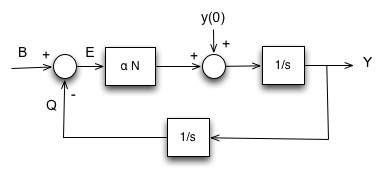
\includegraphics[width=4in]{case1-block.jpg} 
   \caption{Block diagram of the link sharing model}
   \label{fig:case1-block}
\end{figure}

For $\alpha > 0$, this system is marginally stable.
However,  the magnitude of oscillations increases for higher $\alpha$ and/or higher $N$.

This indicates that 
the existence of flows that
rapidly change their sending rates
through high values of $\alpha_i$ 
can cause the system to have high oscillations.
This suggests that elastic flows
that aggressively change their sending rates,
may affect the stability of other flows that
change their sending rates cautiously,
in a system that mixes both kinds of flows.
Furthermore, in such a system,
the value of $N$ may be high so as 
to cause high oscillations.

We now derive the values of the state variables
at equilibrium.
Denote by $x_i$ and
$q$ the steady-state values
of $x_i(t)$ and $q(t)$, respectively.
Then, at equilibrium, we have from Equations~(\ref{app:aggregate-state}):
\begin{eqnarray*}
0 &=&  \alpha (B - q)  \nonumber \\ 
0 &=&  \sum_{j=1}^{N} x_j - C 
\end{eqnarray*}
Thus, at equilibrium, $q = B$ and $\sum_{j=1}^{N} x_j = C$.
In other words,
the system converges to a state where
the total input rate matches the total service rate,
and the target total buffer space is met.

Note that if 
$\alpha_i = \alpha$ for all $i$,
then $x_i(t)$ changes at the same rate
for every flow $i$.
Consequently, if we start the evolution of
the system with $x_i(0)$ being the same
for all flows,
only then we have equal sharing of the network
at steady-state, i.e.\ $x_i = \frac{C}{N}$,
regardless of the initial value $q(0)$.
However, in general,
when $x_i(0)$ are not equal
for all flows,
the system converges to an {\em unfair} state,
more precisely, to a state where
\begin{eqnarray*}
x_i = x_i(0) + \frac{C - \sum_{j=1}^{N} x_j(0)}{N}
\end{eqnarray*}

To summarize,
controlling several flows 
by observing the resulting aggregate state of
the network may lead to high oscillations 
due to either
the existence of flows which
are rapidly adjusting their sending rates,
or a high number of flows competing
for the same {\em shared} resource.
Furthermore, 
the system is highly likely to converge to
an unfair state where flows receive
unequal shares of the resource.


\subsection{Individual Control or Isolation}
\label{sec:individual-control}

Under individual PI control,
the evolution of the system state is described by the following
differential equations:
\begin{eqnarray}
\dot{x}_i(t) &=&  \alpha_i (B_i-q_i(t))  \nonumber \\ 
\dot{q}_i(t) &=&  x_i(t) - c_i(t) 
\label{eqn:individual-state}
\end{eqnarray}

Recall that under individual control,
flow/class $i$ regulates its input, $x_i(t)$,
based on its {\em own} number of outstanding packets.
For simplicity,
assume a constant packet service rate,
i.e.\ $c_i(t) = C_i$ for all $t$.
Following the same stability analysis as aggregate control,
it is easy to see that flow/class $i$ stabilizes and
the poles of the closed-loop system are:\footnote{
We set $N = 1$ in Equation~(\ref{eqn:poles-aggr}).}
\begin{eqnarray*}
	s = \stackrel{+}{-} j \sqrt{\alpha_i}
\label{eqn:individual-stability}
\end{eqnarray*}
Observe that, unlike aggregate control,
flows/classes are {\em isolated} from each other.
Therefore, 
the existence of flows/classes that
rapidly change their sending rates
through high values of $\alpha_i$, 
does not affect the stability of other flows.
This isolation can be implemented using,
for example, a class-based queueing (CBQ) discipline \cite{cbq:1995}.
In such CBQ system,
each class of homogeneous flows can be allocated
its own buffer space and service capacity.

We now derive the values of the state variables
of flow/class $i$
at equilibrium.
Denote by $x_i$ and
$q_i$ the steady-state values
of $x_i(t)$ and $q_i(t)$, respectively.
Then, at equilibrium, we have from Equations~(\ref{eqn:individual-state}):
\begin{eqnarray*}
0 &=& \alpha_i (B_i-q_i) \nonumber \\ 
0 &=&  x_i - C_i
\end{eqnarray*}
Thus, at equilibrium, $q_i = B_i$ and $x_i = C_i$.
In other words,
each flow/class $i$ converges to a state where
its input rate matches its allocated service rate,
and its target buffer space is met.
We note that 
if the allocated buffers $B_i$ and 
service capacities $C_i$ are equal,
then every flow receives an equal share
of the resources,
{\em regardless of} the initial values 
$x_i(0)$ and $q_i(0)$.
One can also achieve a weighted resource sharing
by assigning different $B_i$ and $C_i$ allocations.
Thus, a flow/class with higher priority
(e.g., short interactive TCP flows operating aggressively in slow start)
can be allocated more resources,
so as to receive better throughput/delay service
than other flows (e.g., long TCP flows operating cautiously in congestion avoidance).


To summarize,
controlling each flow (or class of homogeneous flows) 
by observing its own individual state 
within the network 
provides isolation between them.
Thus, stability can be achieved 
for a flow/class regardless of
the behavior and number of other flows/classes.
Furthermore, 
the system can converge to
a fair state where flows/classes receive
a weighted share of the resources.




\section{Case Study: Elastic Transport Tunnel}
\label{sec:case2}

  Consider $n$ regular user connections between sending and receiving
  end-hosts, all passing through two ``gateways" --- let's call them a source gateway and
  a destination gateway.  Our main goal
  is to provide a ``soft bandwidth-guaranteed" tunnel \cite{MinaBestavrosMattaX:iscc04} for these user
  flows over an Internet path of bottleneck capacity $C$, which is
  also shared by another set of $x$ flows, representing cross traffic
  (see Figure~\ref{fig:case2-tunnel}).
  By ``soft" guarantee we mean that there is no explicit resource reservation.
  Consider that user and cross-traffic connections
  are all rate-adaptive connections (similar to TCP). 
  These $x$ cross-traffic connections present a
  challenge: as $x$ keeps changing, the bandwidth allocation for the
  $n$ user flows keeps changing in tandem.  So an important
  question is whether it is possible to ``counter'' the change in $x$
  so as to ensure that the $n$ user flows are able to maintain a
  desirable bandwidth.
  
  \begin{figure}[htbp] %  figure placement: here, top, bottom, or page
     \centering
     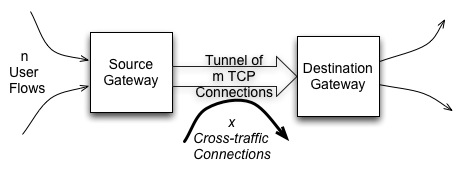
\includegraphics[width=4in]{case2-tunnel.jpg} 
     \caption{Soft bandwidth-guaranteed tunnel}
     \label{fig:case2-tunnel}
  \end{figure}

Clearly without the intervention of the two gateways, the answer to the above
  question is {\em no}. When different flows share a link, the effect
  of each individual flow (or an aggregate of flows) affects the rest
  since all are competing for a fixed amount of resources.  However,
  if the gateways dynamically maintain a number $m$ of open rate-adaptive (e.g., TCP)
  connections between them, they can increase $m$ to provide a positive pressure that
  would equalize the pressure caused by the cross-traffic connections,
  if the latter occurs.  Since $m$ will be changing over time, we
  describe the gateway-to-gateway tunnel, made of the $m$ connections, as {\em elastic}.  Note that the
  source gateway can decide to reduce $m$ (i.e.\ relieve pressure) if $x$
  goes down---the reason is that as long as the tunnel is achieving
  its target bandwidth, releasing extra bandwidth should improve the
  performance of cross-traffic connections, which is in the spirit of
  best-effort networking.


To illustrate this scenario and  the issues involved,
  consider a gateway-to-gateway tunnel going through a single bottleneck
  link.  Assuming long-lived TCP-like load, the behavior of the bottleneck can be
  approximated by Generalized Processor Sharing (GPS) \cite{GPS:1994}, 
  i.e.\ each connection receives the same fair share of resources \cite{Chiu:1989}.
  Thus, each connection ends up with
  $\frac{C}{m+x}$ bandwidth.  This, in turn, gives the $m$ gateway-to-gateway rate-adaptive
  flows, or collectively the elastic gateway-to-gateway tunnel, a bandwidth of
  $\frac{Cm}{m+x}$.  As the source gateway increases $m$ by opening more
  rate-adaptive connections to the destination gateway, the tunnel can grab more
  bandwidth.  If $x$ increases, and the gateways measure a tunnel's
  bandwidth below a target value (say $B^*$), then $m$ is increased to
  push back cross-traffic connections.  If $x$ decreases, and the gateways
  measure a tunnel's bandwidth above $B^*$, then $m$ is decreased for
  the good of cross-traffic connections.  It is important to note that
  the source gateway should refrain from unnecessarily increasing $m$,
  thus achieving a tunnel's bandwidth above $B^*$, since an
  unnecessary increase in the total number of competing rate-adaptive flows
  reduces the share of each connection and may cause flows to
  timeout leading to inefficiency and unfairness.  
  The source gateway also has the responsibility
  of scheduling user packets coming on the $n$ user connections over
  the tunnel, i.e.\ the $m$ gateway-to-gateway connections.
  In this case study, we do not focus on scheduling but the control theoretic 
  modeling and analysis of the tunnel's bandwidth adaptation.
 We study the effect of different types of controllers employed at the source gateway.
 Such controller determines the degree of
elasticity of the gateway-to-gateway rate-adaptive tunnel,
thus it determines
the transient and steady-state behavior of
the soft bandwidth-guaranteed service. \\

\noindent{\bf{Na\"{\i}ve Control:}}
This na\"{\i}ve controller 
measures the bandwidth $b'$ grabbed by 
the current $m'$ gateway-rate-adaptive connections.
Then,
it directly computes the quiescent number $\hat{m}$
of gateway-rate-adaptive  connections that should be open as:
\begin{eqnarray*} 
 \label{eqn:q_m} 
 \hat{m} &=& \frac{B^*}{b'}m'
\end{eqnarray*}

\noindent
Clearly, this controller na\"{\i}vely relies on
the previously measured bandwidth $b'$
and adapts without regard to delays in
measurements and possible changes in network conditions,
e.g.\ changes in the amount of cross traffic.
We thus investigate general well-known controllers
which judiciously zoom-in toward the target bandwidth value.
To that end,
let us develop a flow-level model
of the system dynamics. 
The change in
the bandwidth grabbed $b(t)$ by the $m(t)$ 
gateway-rate-adaptive flows (constituting the elastic gateway-to-gateway tunnel) 
can be described as:
\begin{eqnarray*} 
 \label{eqn:b_dot}    
   \dot b(t) &=&   \alpha [ (C-B^*) m(t) - B^* x(t)]
\end{eqnarray*}

\noindent 
This dynamic equation captures what we want to model:
$b(t)$ increases with $m(t)$, and decreases
as the number of cross-connections $x(t)$ increases. 
$\alpha$ is a constant that represents the degree of multiplexing of
flows and we choose it here to be the steady-state connection's fair share
ratio of the bottleneck capacity. 
At steady-state,
$\dot b(t)$ equals zero, which yields (as expected):
\begin{eqnarray*} 
 \label{eqn:m_x_ss}    
   B^* &=&   \frac{C \hat m} {(\hat x+\hat m)}
\end{eqnarray*}
where $\hat m$ and $\hat x$ represent the steady-state values for the
number of gateway-rate-adaptive flows and cross-traffic flows, respectively.
\noindent
Based of the current bandwidth allocation $b(t)$ and the target
bandwidth $B^*$, an error signal $e(t)$ can be obtained as:
\begin{eqnarray*} 
 \label{eqn:e}    
   e(t) &=&   B^* - b(t)
\end{eqnarray*}

\noindent{\bf{P and PI Control:}}
A controller would adjust $m(t)$ based on the value
of $e(t)$. 
For a simple
Proportional controller (P-type), such adjustment is described by:
\begin{eqnarray} 
 \label{eqn:p}    
   m(t) &=&  K_p e(t)
\end{eqnarray}
\noindent
Recall that P-type controllers are known to result in a non-zero steady-state error.
To exactly achieve the target $B^*$ (i.e.\ with zero steady-state error),
a Proportional-Integral (PI-type) controller can be used:
\begin{eqnarray} 
 \label{eqn:pi}    
   m(t) &=& K_p e(t)+ K_i \int e(t) \ dt
\end{eqnarray}

\noindent
Figure \ref{fig:block1} shows the block diagram 
of this elastic-tunnel model.
In the Laplace domain,
denoting the controller transfer
function by $G_c(s)$, 
the output $B(s)$ is given by:
{\small
\begin{eqnarray} 
 \label{eqn:tf} B(s)= \frac{G_c(s)G_1(s)}{1+G_c(s)G_1(s)} B^*(s) +
   \frac{G_2(s)}{1+G_c(s)G_1(s)} X(s)
\end{eqnarray}
}
where $G_1(s)$ is given by:
\begin{eqnarray*} 
 \label{eqn:g1}    
   G_1(s) &=& \frac{\beta}{s}
\end{eqnarray*}
where $\beta = \alpha (C-B^*)$.
$G_2(s)$ is given by:
\begin{eqnarray*} 
 \label{eqn:g2}    
   G_2(s) &=& \frac{\gamma}{s}
\end{eqnarray*}
where $\gamma = -\alpha B^*$.
\noindent
For the P-controller, 
from Equation~(\ref{eqn:p}), $G_c(s)$ is simply $K_p$.
For the PI-controller, from Equation~(\ref{eqn:pi}),
$C(s)$
equals  $K_p + \frac{K_i}{s}$.
Thus,
the transfer function $\frac{B(s)}{B^*}$ 
in the presence of a  P-controller
is given by:
\begin{eqnarray*} 
 \label{eqn:tfp}    
    \frac{B(s)}{B^*} &=& \frac{K_p \beta}{s + K_p \beta}
\end{eqnarray*}
The system with P-controller is always stable
since the root of the characteristic equation 
(i.e.\ the denominator of the transfer function) is
negative, given by $-K_p \beta$ for $\beta > 0$ and $B^* < C$.
\noindent
In the presence of a PI-controller,
the transfer function $\frac{B(s)}{B^*}$ 
is given by: 
\begin{eqnarray*} 
 \label{eqn:tfpi} 
 \frac{B(s)}{B^*} &=& \frac{K_p\beta s + K_i\beta}
{s^2 + K_p\beta s + K_i\beta}
\end{eqnarray*}
One can choose the PI-controller parameters
$K_p$ and $K_i$ to achieve a certain convergence
behavior to the target bandwidth $B^*$.
We next define transient performance measures
to assess such convergence behavior.

\begin{figure}[htbp] %  figure placement: here, top, bottom, or page
   \centering
   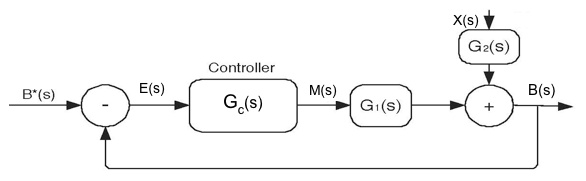
\includegraphics[width=4in]{tunnel-block1} 
\caption{Block diagram of the elastic-tunnel model} 
\label{fig:block1}
\end{figure}

\subsection{Transient Performance}
Transient behavior represents the system's response 
which decays with
time. 
In the design of reliable systems,
it is extremely important 
that transient response meets certain requirements, 
e.g.\ reasonable settling time and overshoot (cf.\ Section~\ref{sec:transient}). 
Often times, the transient response is
obtained by subjecting the system to an impulse or a step input and
observing the output(s).
One has to guarantee that the response of the
system to specific inputs does not render the system
unstable or pushes it away from its intended target.

Figure~\ref{fig:trans1} shows
 the step response of the
transfer function given in
Equation~(\ref{eqn:tf}).
The left column 
shows  the response to a unit step change
in the target bandwidth, while the right column 
shows the
response to a unit step change in the cross-traffic. 
Figure~\ref{fig:trans1}(a),
for the P-controller,
shows that while the response could be acceptable due to
a step change in the reference bandwidth (i.e., the response $b(t)$ achieves the unit target), 
it fails to remove the steady-state
error (i.e., non-zero $b(t)$) obtained from the step change in the cross-traffic. 
Figures~\ref{fig:trans1}(b) and~(c)
show the response due to the PI-controller. 
One can
see that through a careful choice of $K_p$ and $K_i$, the transient
response can be adjusted.  
Notice that with a PI-controller,
the elastic-tunneling system can reach the target bandwidth with
zero steady-state error in response to a step change
in cross-traffic.



\begin{figure*}[thbp]
\begin{center} 
\begin{minipage}{0.4\textwidth} 
   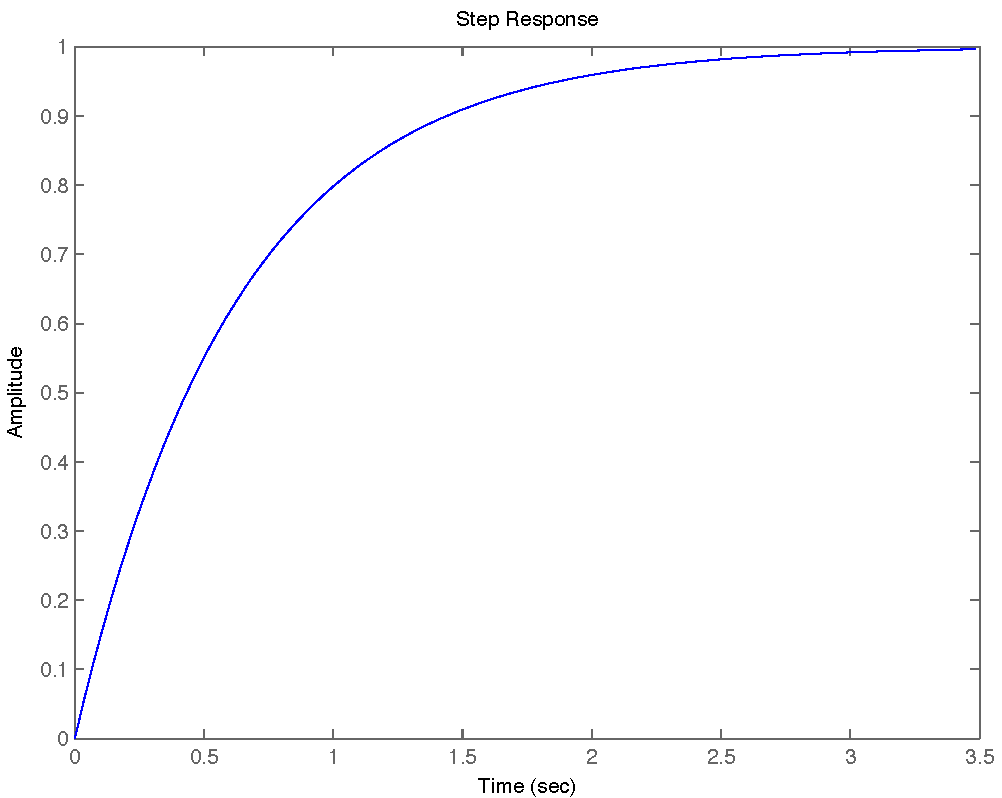
\includegraphics[width=2.5in]{plots/trans/P_step_B_01.pdf} 
\centerline{Target Bandwidth Step Response}
\end{minipage}
\hspace{1.2cm}
\begin{minipage}{0.4\textwidth} 
   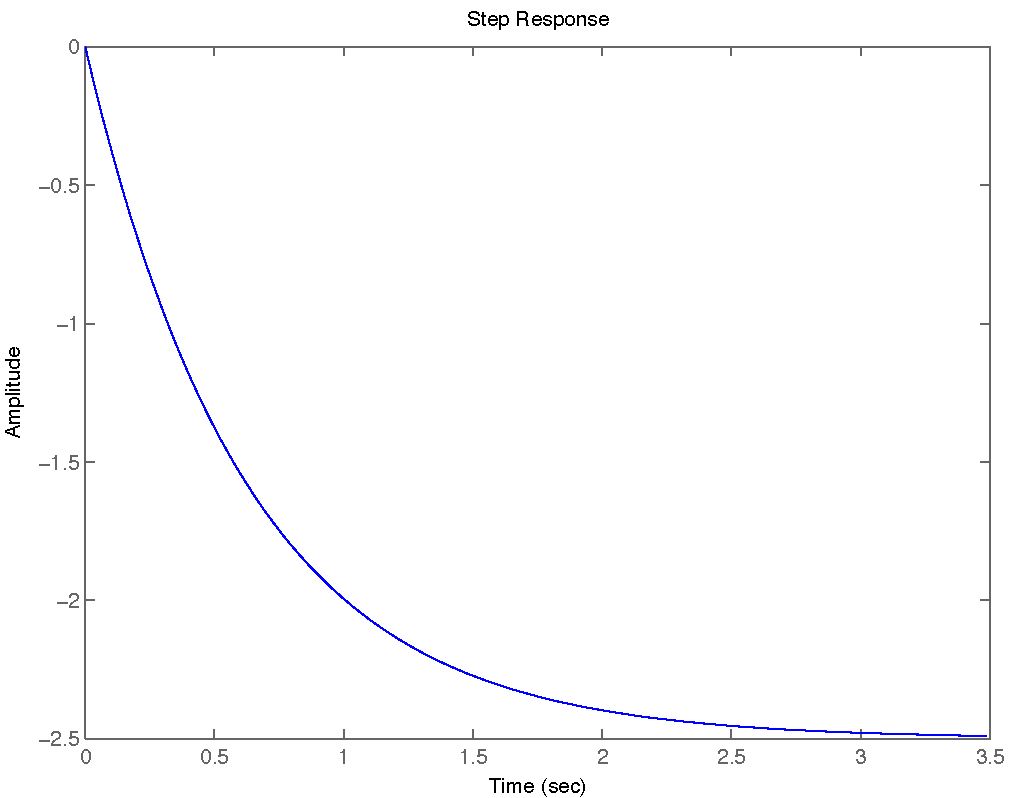
\includegraphics[width=2.5in]{plots/trans/P_step_x_01.pdf} 
\centerline{Cross-traffic Step Response}
\end{minipage}
\centerline{(a) Proportional controller with $K_p$ = 0.1}\\

\begin{minipage}{0.4\textwidth} 
   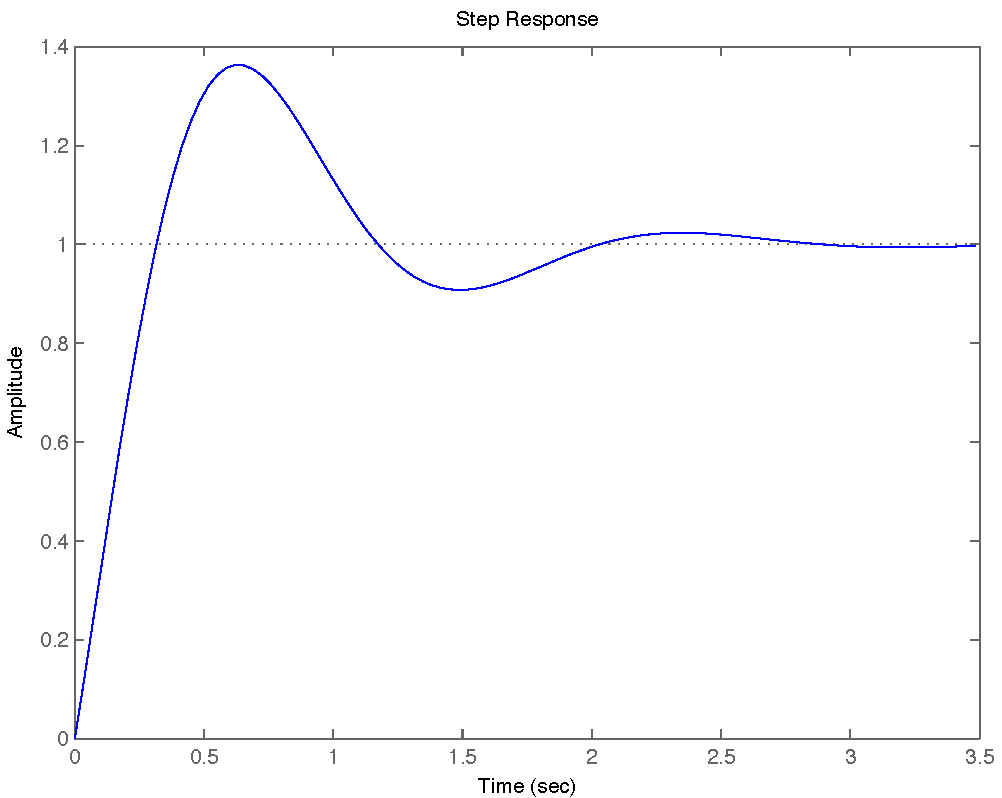
\includegraphics[width=2.5in]{plots/trans/PI_step_B_02_1.pdf} 
\centerline{Target Bandwidth Step Response}
\end{minipage}
\hspace{1.2cm}
\begin{minipage}{0.4\textwidth} 
   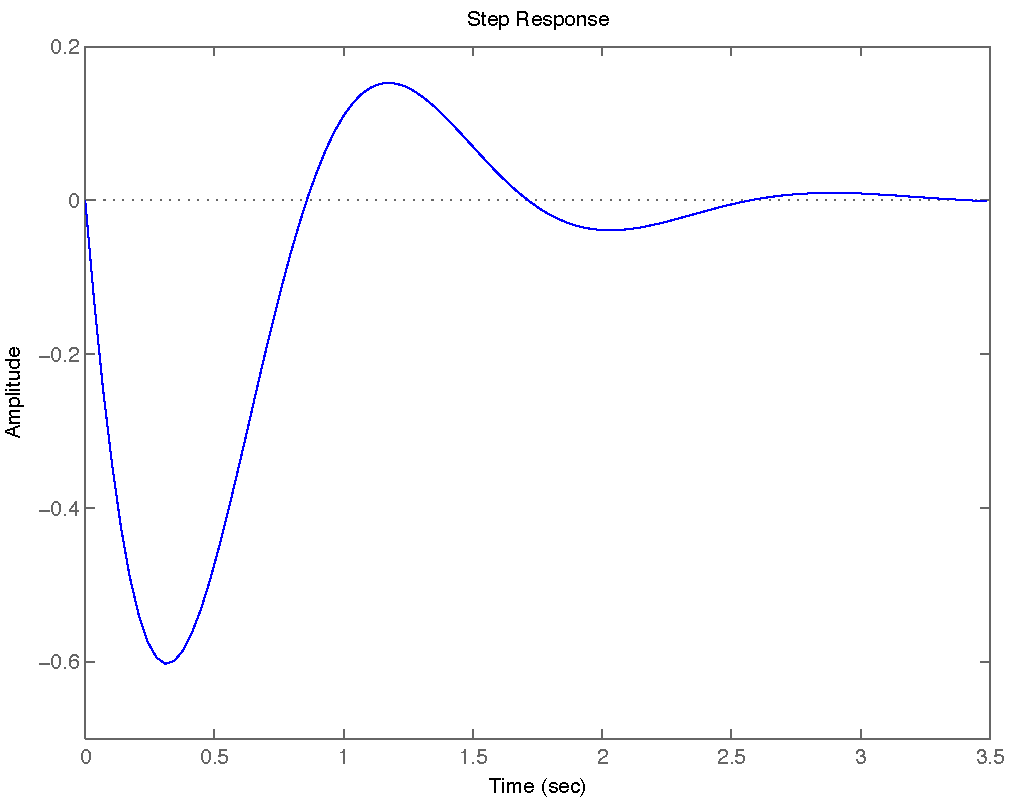
\includegraphics[width=2.5in]{plots/trans/PI_step_x_02_1.pdf} 
\centerline{Cross-traffic Step Response}
\end{minipage}
\centerline{(b) Proportional Integral controller with $K_p$ = 0.2 and $K_i$ = 1}\\

\begin{minipage}{0.4\textwidth} 
   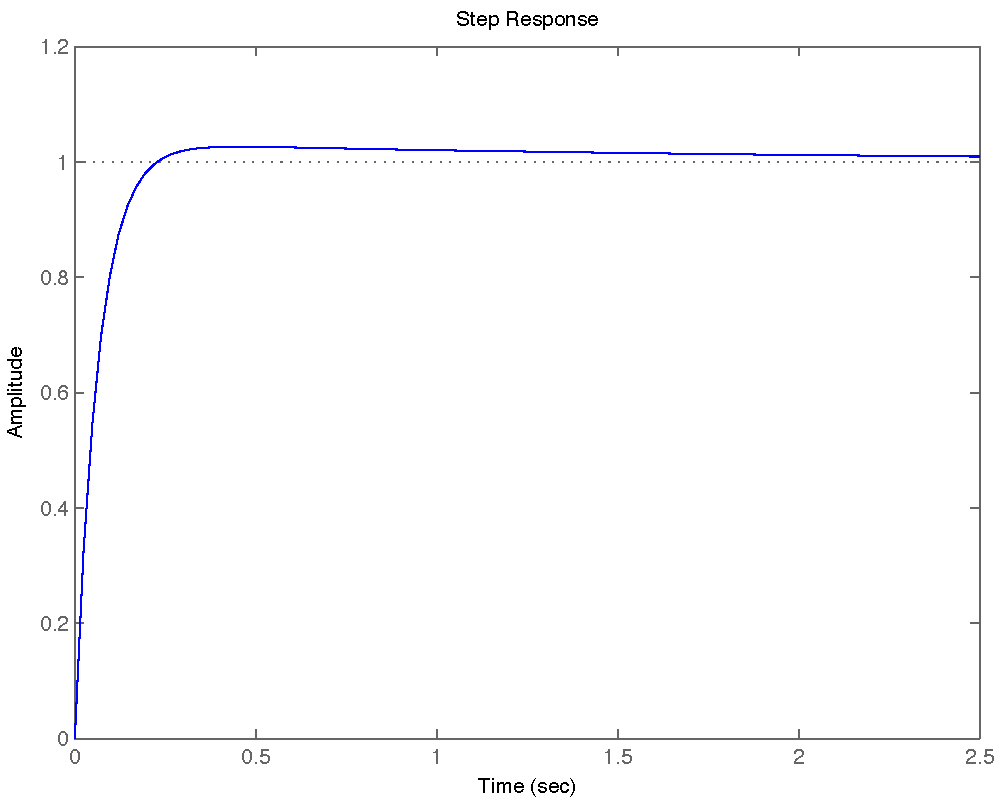
\includegraphics[width=2.5in]{plots/trans/PI_step_B_1_05.pdf} 
\centerline{Target Bandwidth Step Response}
\end{minipage}
\hspace{1.2cm}
\begin{minipage}{0.4\textwidth} 
   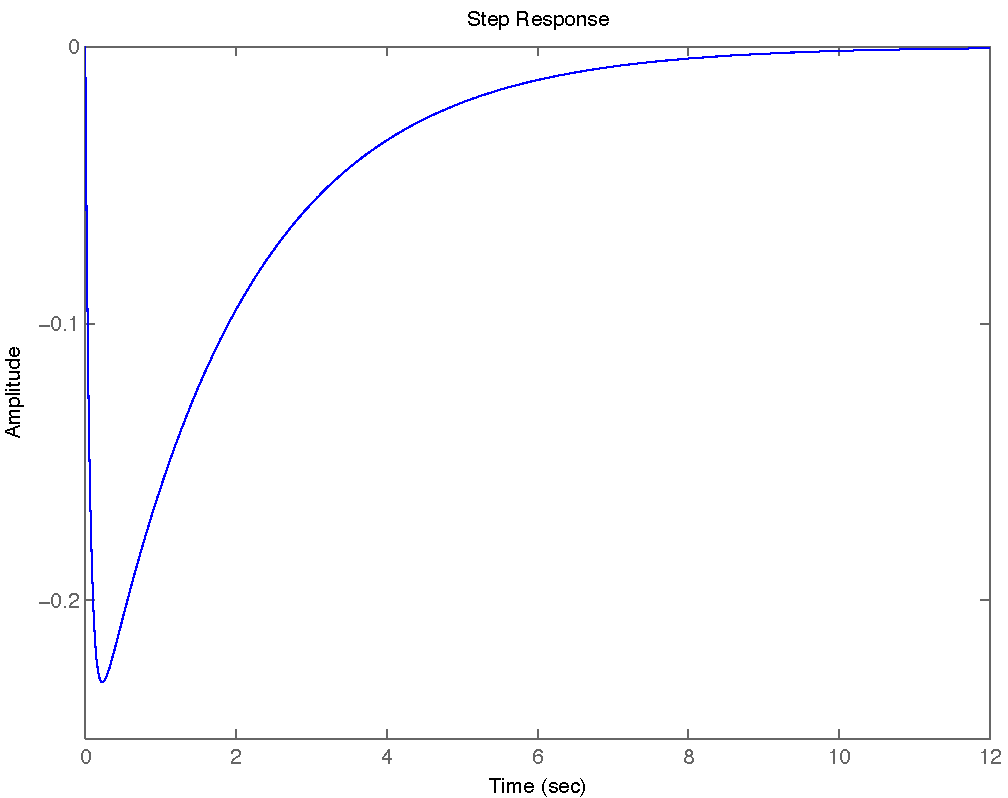
\includegraphics[width=2.5in]{plots/trans/PI_step_x_1_05.pdf} 
\centerline{Cross-traffic Step Response}
\end{minipage}
\centerline{(c) Proportional Integral controller with $K_p$ = 1 and $K_i$ =
0.5}\\
\caption{Transient analysis of the elastic-tunnel model}
\label{fig:trans1} 
\end{center}
\end{figure*}

\begin{figure}[tbp]
   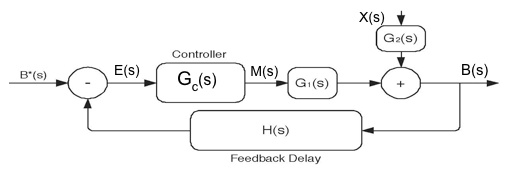
\includegraphics[width=5in]{tunnel-block} 
\caption{Elastic-tunnel model (with feedback delay)} 
\label{fig:block2}
\end{figure}

\subsection{Effect of Feedback Delay}
So far in our analysis, we have ignored the feedback delay which is
inherent in the design of any control system 
that tries to adjust its signal through
a delayed feedback loop.


Figure~\ref{fig:block2} augments the block diagram
of Figure~\ref{fig:block1}
with feedback delay denoted by $H(s)$. 
This feedback
delay arises either due to delayed
mesurements of bandwidth and/or
delayed response of the system as a result of
applying new control.
For example, when 
a new gateway-rate-adaptive connection is opened, 
it doesn't get its steady-state throughput instantaneously,
rather after some delay (say $\tau$). Thus, $H(s)$ is given by:
\begin{eqnarray*} 
 \label{eqn:hs}    
   H(s) &=& e^{-\tau s}
\end{eqnarray*}
where $\tau$ represents the feedback time delay.
For small $\tau$, the above
equation can be approximated by:
\begin{eqnarray*} 
 \label{eqn:ahs}    
   H(s) &\approx& 1 - \tau s
\end{eqnarray*}
If we are using a PI-controller, the characteristic equation in 
the presence
of feedback delay becomes:
\begin{eqnarray*} 
 \label{eqn:cch}    
    s^2(1-\beta \tau K_p) + s(K_p\beta - \beta \tau K_i) + \beta K_i = 0
\end{eqnarray*}


Figure~\ref{fig:trans2} shows the response
of the PI-controller to a unit step change in the target bandwidth.
As the feedback delay $\tau$ increases,
the system may not converge to the target bandwidth.


\begin{figure*}[htbp]
\begin{center} 
\begin{minipage}{0.4\textwidth} 
   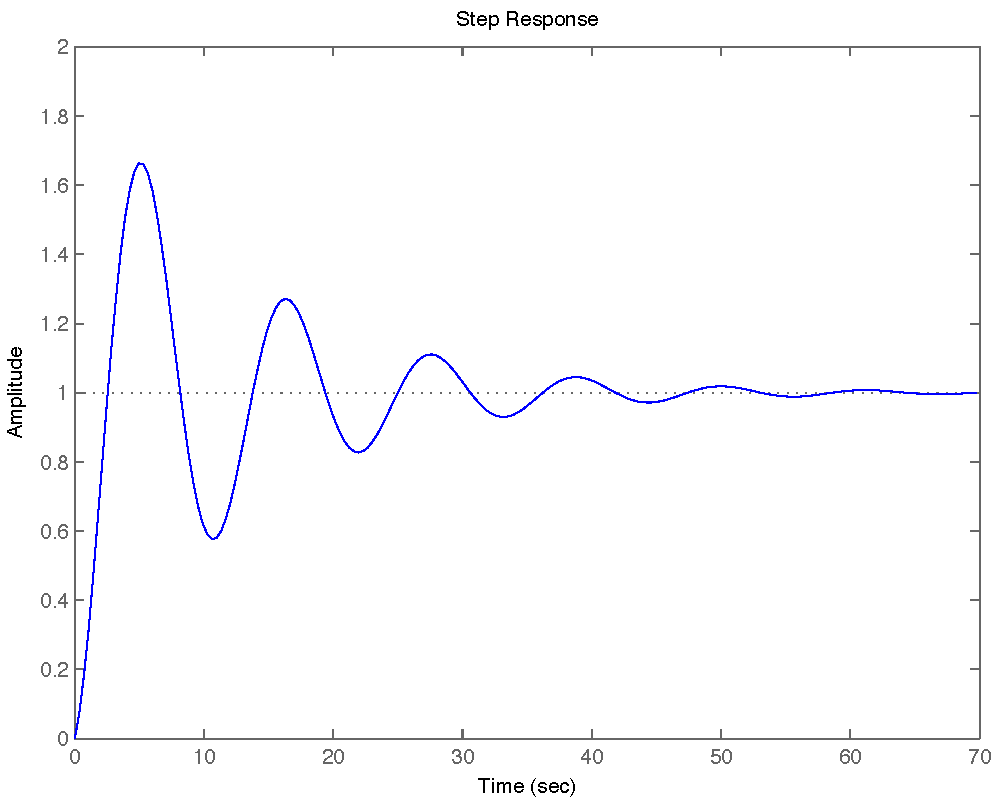
\includegraphics[width=2.5in]{plots/trans/PI_step_B_001_002.pdf} 
\centerline{Target Bandwidth Step Response}
\end{minipage}
\hspace{1.2cm}
\begin{minipage}{0.4\textwidth} 
   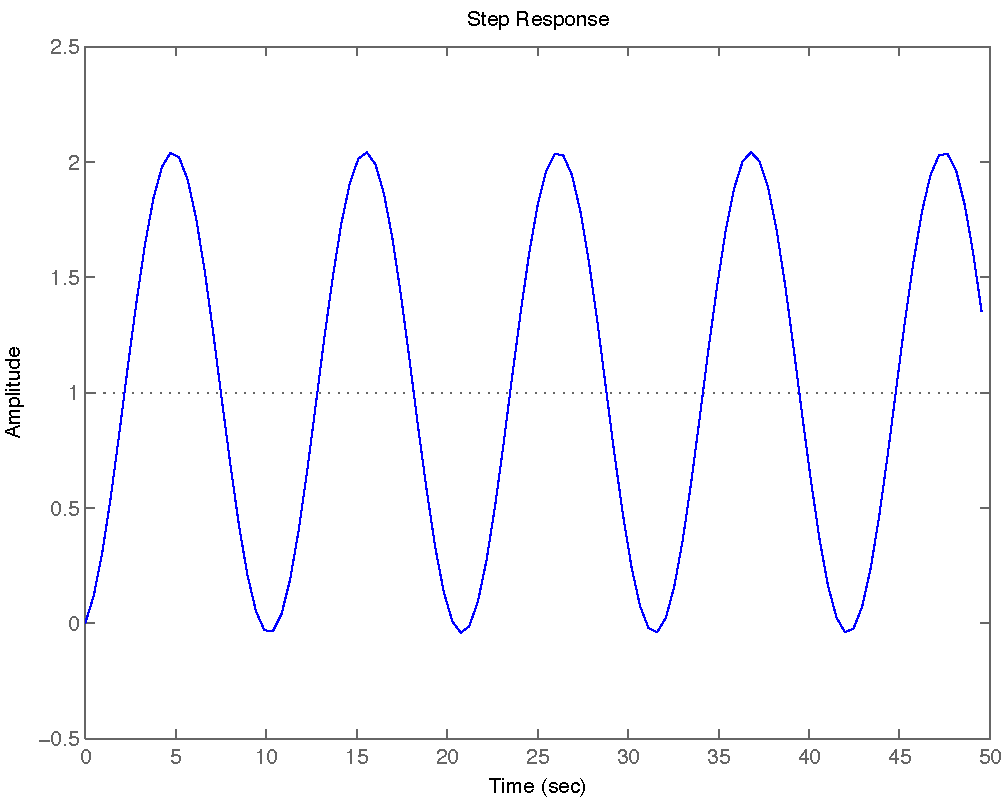
\includegraphics[width=2.5in]{plots/trans/PI_step_B_001_002_delay_05.pdf}  
\centerline{Response with Feedback Delay}
\end{minipage}
\centerline{Proportional Integral controller with $K_p$ = 0.01 and
$K_i$ = 0.02}\\
\caption{Transient analysis of the elastic-tunnel model (with feedback delay)}
\label{fig:trans2} 
\end{center}
\end{figure*}




\section{Exercises}
\label{sec:exercises}

\begin{enumerate}

\item Let $r$ be a max-min fair rate vector corresponding to a given network and set of flows. This max-min fair allocation maximizes the allocation of each flow $i$ subject to the constraint that an incremental increase in $i$'s allocation does not cause a decrease in some other flow's allocation that is already as small as $i$'s or smaller.

\begin{itemize}
\item[(a)] Suppose that some of the flows are eliminated and let $\bar{r}$ be a corresponding max-min fair rate vector. Show by example that we may have $\bar{r}_p < r_p$ for some of the remaining flows $p$.

\item[(b)] Suppose that some of the link capacities are increased and let $\bar{r}$ be a corresponding max-min fair rate vector. Show by example that we may have  $\bar{r}_p < r_p$ for some flows $p$.
\end{itemize}

\item Consider two network links in tandem (one after the other) of capacities 6 Mbps each. For two different sets of elastic flows (i.e. the utility function of each flow/user is a log function of its allocated rate), you are asked to write down the corresponding network optimization problem, where the network tries to maximize the sum of flow utilities subject to link capacity constraints. For each set of flows, described in parts (a) and (b) below, rewrite the constrained optimization problem as an unconstrained optimization problem: write down the Lagrangian function and corresponding equations to solve for the optimal rate allocation. What are the optimal rates allocated to different flows for each one of these two settings?
\begin{itemize}
\item[(a)] Consider two flows: one flow using the first link only and another flow using both links.

\item[(b)] Consider the same two flows from part (a), as well as a third flow using the second link only.
\end{itemize}

\item  Consider two network links in tandem (one after the other) of capacities 6 Mbps each. 
Assume three flows: one flow using the first link only, another flow  using the second link only,
and a third flow using both links.
Assume the utility function of each flow/user is a log function of its allocated rate, 
and that the two-link flow is given a weight of 2, while the two one-link flows are given a weight of 1.

You are asked to write down the corresponding network optimization problem, where the network tries to maximize the sum of the weighted flow utilities subject to link capacity constraints.  Rewrite the constrained optimization problem as an unconstrained optimization problem: write down the Lagrangian function and corresponding equations to solve for the optimal rate allocation. What are the optimal rates allocated to each flow? 


\item Consider a source adapting its sending rate $x(t)$ so the buffer size of  its path's bottleneck $b(t)$ stays at a certain target value $T$. Denote the error signal by  $e(t) = T-b(t)$. The sending rate is adapted according to one of the following three controllers:
\begin{enumerate}
\item $x(t)=K_p  e(t)$   

\item $x(t)= K_p  e(t)+ K_i \int_0^t e(t)dt$ 

\item $x(t)= K_p  e(t)+ K_i \int_0^t e(t)dt+ K_d  \frac{d}{dt} e(t)$  
\end{enumerate}
where  $K_p, K_i, K_d$   are constant parameters of the rate controllers.

\begin{itemize}
\item[(a)] Assume $c(t)$ is the capacity available to the source at time $t$, write down the differential equation for $b(t)$.

\item[(b)] By transforming the system to the Laplace domain, determine the conditions under which the system is stable for each type of controller, i.e. does $b(t)$ converge to a given $T$ for certain values of $K_p, K_i, K_d$. Do this by examining the roots (poles) of the characteristic equation of the system's transfer function. Draw the block diagram of the system that shows the relationships between the system variables in the (Laplace) s-domain for each type of controller.

\item[(c)] Again by examining the roots (poles) of the characteristic equation of the system's transfer function and using the Final Value Theorem, compare the transient and steady-state performance under each type of controller.

\item[(d)] Support your answers above by numerically solving the system's equations over time for each type of controller. Assume a small time step $\Delta$, say $\Delta=1$, and solve the discretized version of the equations at these time steps -- you can then approximate the differentiation $\frac{d}{dt} b(t)$ by $b(t)-b(t-1)$.
\end{itemize}


\item Consider an adaptation of a transmission window $w$ whose goal is to reach a target window $T$ as follows:
\begin{eqnarray*}
w_{(k+1)} =  w_k+ \alpha(T-w_k)
\end{eqnarray*}
where  $0 < \alpha < 1$. 
\begin{itemize}
\item[(a)] Derive the necessary condition (if any) for convergence to the target window size.
\item[(b)] Use the Lyapunov method to show whether the system converges regardless of the initial window size.
\end{itemize}

\item Given a system with the following adaptation rules: $x(t)$, representing a sending rate, is adapted using an AIMD policy, whereas $p(t)$, representing the price, is adapted in proportion to how far $x(t)$ is from a target capacity $c$:

\begin{eqnarray*}
\frac{d x(t)}{dt} = 1- x(t) p(x(t)) 
\end{eqnarray*}

\begin{eqnarray*}
p(x(t))= \alpha (x(t)-c)
\end{eqnarray*}

\begin{itemize}
\item[(a)] Why is that system non-linear?

\item[(b)] Linearize the system around a certain operating point $x_0$. 

\item[(c)] By transforming the linearized system to the Laplace domain, obtain the condition on $x_0$ under which the linearized system is stable.
\end{itemize}


\item 

This question is based on the paper {\em The Revised ARPANET
Routing Metric, by Zinky and Khanna} \cite{Khanna:1989}.
A unified way to model adaptive resource
management---whether it is TCP adaptive to RED or routing adaptive
to changing link costs or other examples---is through two
functions: a feedback (pricing) function such as that of RED or
link utilization metric, and an adaptation function such as that
of TCP or utilization-based routing. Consider a resource that
generates prices $p$ and users that adapt their load $\lambda$
based on the currently reported $p$. Assume the following pricing
and load adaptation functions: \begin{center} $\lambda = 1 - p$
\end{center} \[ p = \left\{ \begin{array}{ll}
       0.1 & \mbox{if $ 0 \leq \lambda < 0.4$} \\
       0.2  & \mbox{if $ 0.4 \leq \lambda \leq 0.8$} \\
       1.0  & \mbox{if $ 0.8 < \lambda \leq 1.0$}
       \end{array}
\right. \]

Show the two functions on the ($\lambda, p$) plane. Trace one
trajectory showing convergence to a fixed point, and another
trajectory showing oscillations. {\em Hint:} consider initial
values of $\lambda$ = 0.2 and 0.6.



\end{enumerate}


\section{Solutions to Exercises}
\label{sec:solutions}

\begin{enumerate}

\item 


\begin{itemize}
\item[(a)] Refer to Figure \ref{fig:max-min-alloc}. Using max-min fairness the original
flow assignment is: (F1=50, F2=50, F3=50, F4=100). Assume F2 is
removed. The new assignment is: (F1=75, F2=0, F3=75, F4=75). F1
and F3 will share the extra capacity, while F4 will decrease its
rate. This is only possible because F4's original assigned rate
was not less than or equal to F3's rate, before F2 was removed,
thus allowing F3 to increase its rate. 

\item[(b)] Refer to Figure \ref{fig:max-min-alloc}. Using max-min fairness the original
flow assignment is: (F1=50, F2=50, F3=50, F4=100). If the capacity
of link 1 is increased to 225 then the new allocated rates will
be: (F1=75, F2=75, F3=75, F4=75). The extra capacity on link 1
will be shared by F1, F2 and F3. Again, this is only possible
because F4's original assigned rate is not less than or equal to
F3's rate, before the capacity of link 1 was increased, thus
allowing F3 to increase its rate. 
\end{itemize}

\item

Note that earlier in these notes, we did not explicitly cover the technique of ``slack",
which we use here to denote residual link capacity when solving the dual Lagrangian problem.
Intuitively, if the link is fully utilized, i.e. it has zero slack,
then its price (Lagrangian multiplier) is non-zero.
On the other hand, a non-bottleneck link will have a non-zero slack
and so a price of zero.

\begin{itemize}
\item[(a)] Let $z_1^2$ and $z_2^2$ denote the (non-negative) slack on links 1 and
2, respectively. Let $x_1$ and $x_2$ denote the rates assigned to
flows 1 and 2, respectively. Let $f(x_1, x_2)$ denote the function
to be maximized.

\vspace{-3mm}

\begin{eqnarray*}
f(x_1, x_2) = \lg ~x_1 + \lg ~x_2
\end{eqnarray*}

\noindent Constraints on links 1 and 2, respectively, are as
follows:

\vspace{-5mm}

\begin{eqnarray*}
x_1 + x_2 + z_1^2 - c_1 = 0
\end{eqnarray*}

\vspace{-5mm}

\begin{eqnarray*}
x_2 + z_2^2 - c_2 = 0
\end{eqnarray*}


\noindent Replacing $c_1$ and $c_2$ with their values we get:

\vspace{-5mm}

\begin{eqnarray*}
x_1 + x_2 + z_1^2 - 6 = 0
\end{eqnarray*}

\vspace{-5mm}

\begin{eqnarray*}
x_2 + z_2^2 - 6 = 0
\end{eqnarray*}

\noindent The Lagrangian function to be differentiated is as
follows:

\vspace{-3mm}

\begin{eqnarray*}
F(x_1, x_2) = \lg ~x_1 + \lg ~x_2 - \lambda (x_1 + x_2 + z_1^2 -
6) - \mu(x_2 + z_2^2-6)
\end{eqnarray*}

\noindent Taking the partial derivative with respect to each
variable we get the following equations:

\begin{eqnarray*}
\pd{F}{x_1} = {\frac {1}{x_1}} - \lambda = 0
\end{eqnarray*}

\begin{eqnarray*}
\pd{F}{x_2} = {\frac {1}{x_2}} - \lambda - \mu = 0
\end{eqnarray*}

\begin{eqnarray*}
\pd{F}{\lambda} = -(x_1 + x_2 + z_1^2 - 6) = 0
\end{eqnarray*}

\begin{eqnarray*}
\pd{F}{\mu} = -(x_2 + z_2^2 - 6) = 0
\end{eqnarray*}

\begin{eqnarray*}
\pd{F}{z_1} = -2z_1\lambda = 0
\end{eqnarray*}

\begin{eqnarray*}
\pd{F}{z_2} = -2z_2\mu = 0
\end{eqnarray*}



\noindent
Since F1 can utilize any left over capacity (slack) on
link 1, $z_1 = 0$, which implies that $\lambda \ne 0$.
Conversely, since F2 is limited by link 1, $z_2 \ne 0$, which
implies that $\mu = 0$. \bigbreak

\noindent Replacing $z_1 = 0$ and $\mu = 0$ into the derived
equations, we get:

\vspace{-3mm}

\begin{eqnarray*}
{\frac{1}{x_1}} - \lambda = 0
\end{eqnarray*}

\vspace{-5mm}

\begin{eqnarray*}
{\frac{1}{x_2}} - \lambda - 0 = 0
\end{eqnarray*}

\vspace{-5mm}

\begin{eqnarray*}
x_1 + x_2 + 0 -6 = 0
\end{eqnarray*}


\noindent Solving for $x_1$ we get $x_1 =
{\frac{1}{\lambda}}$

\noindent Solving for $x_2$ we get $x_2 =
{\frac{1}{\lambda}}$. Hence, $x_1 = x_2$.

\noindent Replacing $x_2$ by $x_1$ in the capacity equation we get:

\vspace{-5mm}

\begin{eqnarray*}
x_1 + x_1 = 6
\end{eqnarray*}

\noindent Hence, $x_1 = x_2 = 3.$ \bigbreak

%%%%%%%%%%%%%%%%

\item[(b)] Let $z_1^2$ and $z_2^2$ denote the slack on links 1 and
2, respectively. Let $x_1$, $x_2$ and $x_3$ denote the rates
assigned to flows 1, 2 and 3, respectively. Let $f(x_1, x_2, x_3)$
denote the function to be maximized.

\vspace{-3mm}

\begin{eqnarray*}
f(x_1, x_2, x_3) = \lg ~x_1 + \lg ~x_2 + \lg ~x_3
\end{eqnarray*}

\noindent Constraints on links 1 and 2, respectively, are as
follows:

\vspace{-5mm}

\begin{eqnarray*}
x_1 + x_2 + z_1^2 - c_1 = 0
\end{eqnarray*}

\vspace{-5mm}

\begin{eqnarray*}
x_3 + x_2 + z_2^2 - c_2 = 0
\end{eqnarray*}


\noindent Replacing $c_1$ and $c_2$ with their values we get:

\vspace{-5mm}

\begin{eqnarray*}
x_1 + x_2 + z_1^2 - 6 = 0
\end{eqnarray*}

\vspace{-5mm}

\begin{eqnarray*}
x_3 + x_2 + z_2^2 - 6 = 0
\end{eqnarray*}

\noindent The Lagrangian function to be differentiated is as
follows:

\vspace{-5mm}

\begin{eqnarray*}
F(x_1, x_2, x_3) = \lg ~x_1 + \lg ~x_2 + \lg ~x_3 - \lambda (x_1 +
x_2 + z_1^2 - 6) - \mu(x_3 + x_2 + z_2^2 - 6)
\end{eqnarray*}

\noindent Taking the partial derivative with respect to each
variable we get the following equations:

\begin{eqnarray*}
\pd{F}{x_1} = {\frac {1}{x_1}} - \lambda = 0
\end{eqnarray*}

\begin{eqnarray*}
\pd{F}{x_2} = {\frac {1}{x_2}} - \lambda - \mu = 0
\end{eqnarray*}

\begin{eqnarray*}
\pd{F}{x_3} = {\frac {1}{x_3}} - \mu = 0
\end{eqnarray*}

\begin{eqnarray*}
\pd{F}{\lambda} = -(x_1 + x_2 + z_1^2 - 6) = 0
\end{eqnarray*}

\begin{eqnarray*}
\pd{F}{\mu} = -(x_3 + x_2 + z_2^2 - 6) = 0
\end{eqnarray*}

\begin{eqnarray*}
\pd{F}{z_1} = -2z_1\lambda = 0
\end{eqnarray*}

\begin{eqnarray*}
\pd{F}{z_2} = -2z_2\mu = 0
\end{eqnarray*}

\noindent From the equations above we can deduce the following:

\vspace{-3mm}

\begin{eqnarray*}
x_1 = {\frac{1}{\lambda}}
\end{eqnarray*}

\vspace{-3mm}

\begin{eqnarray*}
x_2 = {\frac{1}{\lambda + \mu}}
\end{eqnarray*}

\vspace{-3mm}

\begin{eqnarray*}
x_3 = {\frac{1}{\mu}}
\end{eqnarray*}

\noindent Since F1 and F3 can utilize any left over capacity
(slack) on links 1 and 2, $z_1 = z_2 = 0$. This implies that
$\lambda \ne 0$ and $\mu \ne 0$. \bigbreak

\noindent Replacing $z_1 = 0$ and $z_2 = 0$ into the derived
equations we get:

\vspace{-3mm}

\begin{eqnarray*}
x_1 + x_2 = 6
\end{eqnarray*}

\vspace{-3mm}

\begin{eqnarray*}
x_2 + x_3 = 6
\end{eqnarray*}

\noindent Replacing $x_1$ by ${\frac{1}{\lambda}}$, $x_2$ by
${\frac{1}{\lambda + \mu}}$ and $x_3$ by ${\frac{1}{\mu}}$ into
the equations above, we get:

\vspace{-3mm}

\begin{eqnarray*}
{\frac{1}{\lambda}} + {\frac{1}{\lambda + \mu}}  = 6
\end{eqnarray*}

\vspace{-3mm}

\begin{eqnarray*}
{\frac{1}{\lambda + \mu}} + {\frac{1}{\mu}}  = 6
\end{eqnarray*}

\noindent Multiplying the first equation by (-1) and adding it to
second equation, results in the following:

\vspace{-3mm}

\begin{eqnarray*}
{\frac{1}{\mu}} - {\frac{1}{\lambda}}  = 0
\end{eqnarray*}

\noindent Hence, $\lambda = \mu$ \bigbreak

\noindent Thus, $x_1 = x_3 = {\frac{1}{\lambda}}$ and $x_2 =
{\frac{1}{2\lambda}} = {\frac{x_1}{2}} = {\frac{x_3}{2}}$

\noindent Finally we get:

\vspace{-3mm}

\begin{eqnarray*}
x_1 + {\frac{x_1}{2}} = 6
\end{eqnarray*}

\noindent Hence, $x_1 = x_3 = 4$ and $x_2 = 2.$

\end{itemize}

%%%%%% answer to exercise 3
\item The objective function we want to maximize is:

$F(x) = \lg\ x_1 + \lg\ x_2 + 2\ \lg\ x_3$

\noindent subject to the capacity constraints:

$x_1 + x_3 \leq 6$ \\
$x_2 + x_3 \leq 6$ \\
$x_1, x_2, x_3 \geq 0$

The Lagrangian (unconstrained) function that we want to maximize is:

$L(x) = \lg\ x_1 + \lg\ x_2 + 2\ \lg\ x_3 - \lambda_1(x_1 + x_3 - 6) - \lambda_2(x_2 + x_3 - 6)$

Note that we do not explicitly include the slacks for the link capacities here, since both links should be fully utilized as the one-link flows are not limited by any other link, so the slack values are zero.

Taking the partial derivatives of $L(.)$ we obtain:

$\pd{L}{x_1} = \frac{1}{x_1} - \lambda_1 = 0 \Rightarrow x_1 = \frac{1}{\lambda_1} $

$\pd{L}{x_2} = \frac{1}{x_2} - \lambda_2 = 0 \Rightarrow x_2 = \frac{1}{\lambda_2} $

$\pd{L}{x_3} = \frac{2}{x_3} - (\lambda_1 + \lambda_2) = 0 \Rightarrow x_3 = \frac{2}{\lambda_1 + \lambda_2} $

$\pd{L}{\lambda_1} = 0  \Rightarrow x_1 + x_3 - 6 = 0 \Rightarrow x_1 + x_3 = 6 $

$\pd{L}{\lambda_2} = 0  \Rightarrow x_2 + x_3 - 6 = 0 \Rightarrow x_2 + x_3 = 6 $

The last two equations yield $x_1 = x_2  \Rightarrow \lambda_1 =  \lambda_2 = \lambda$

From the capacity equation, we have:

$x_1 + x_3 = \frac{1}{\lambda} + \frac{2}{2\lambda} = 6 \Rightarrow \lambda = \frac{1}{3}$, thus

$x_1 = x_2 = 3$, and $x_3 = 6 - 3 = 3. $

%%%%%%%

\item \noindent We use the following notation: \smallbreak

\noindent In the time domain we have:\\
\noindent $b(t)$, buffer size at time $t$\\
\noindent $x(t)$, sending rate at time $t$\\
\noindent $c(t)$, service rate at time $t$\\
\noindent $T$, target buffer size\\
\noindent $e(t)$, error (difference between current buffer size
and the target) at time $t$ \bigbreak

\noindent In the frequency domain we have:\\
\noindent $B(s)$, current buffer size\\
\noindent $X(s)$, sending rate\\
\noindent $C(s)$, service rate\\
\noindent $T(s)$, target buffer size\\
\noindent $E(s)$, error signal\\
\noindent $D(s)$, controller (based on error signal computes
sending rate) \bigbreak

\noindent We will assume that the target buffer size and the
buffer's service rate are constant values.


%%%%%%%%%%%%%%%%%%%%%%%%%%%%
%Question One Part a
%%%%%%%%%%%%%%%%%%%%%%%%%%%%
\bigbreak \bigbreak

\begin{itemize}

\item[(a)] \smallbreak

\noindent $e(t) = T - b(t)$\\
\noindent ${\frac{d}{dt}} b(t) = x(t) - c(t)$


%%%%%%%%%%%%%%%%%%%%%%%%%%%
%Question One Part b
%%%%%%%%%%%%%%%%%%%%%%%%%%%%
\bigbreak \bigbreak

\item[(b)] \smallbreak

\begin{figure*}[htp]
\centerline{
  % Requires \usepackage{graphicx}
  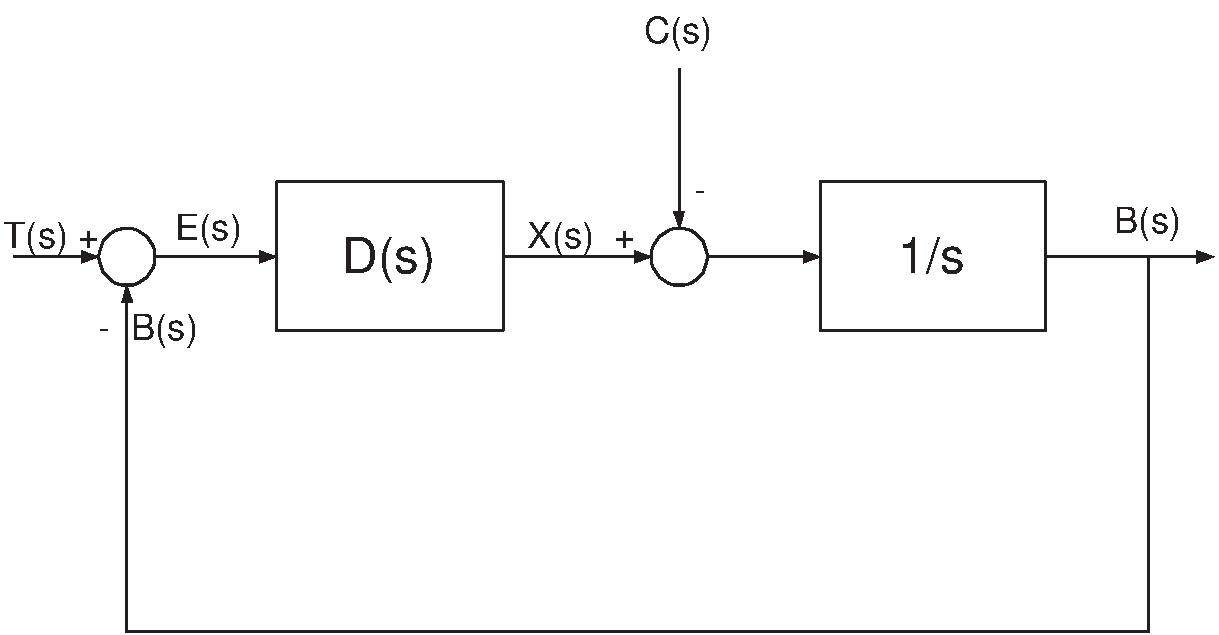
\includegraphics[width=0.7\textwidth]{blockDiagram}
  }
   \caption{System block diagram}
   \label{fig:sol-block}
\end{figure*}

\noindent The system's block diagram is depicted in Figure~\ref{fig:sol-block}.
Using the block diagram, we can formulate the following equation:
\bigbreak

\noindent $~( ~[ ~(T(s) - B(s)) ~D(s)~] - C(s)~) ~({\frac{1}{s}}) = B(s)$\\

\noindent $~( ~[T(s)D(s) - B(s)D(s)] - C(s)~) ~({\frac{1}{s}}) = B(s)$\\

\noindent $~(T(s)D(s) - B(s)D(s) - C(s)) ~({\frac{1}{s}}) = B(s)$\\

\noindent $[{\frac{T(s) D(s)}{s}} - {\frac{B(s) D(s))}{s}} -
{\frac{C(s)}{s}}] = B(s)$\\

\noindent $B(s) + {\frac{B(s) D(s)}{s}} = {\frac{T(s) D(s)}{s}} -
{\frac{C(s)}{s}}$\\

\noindent $B(s)[1 + {\frac{D(s)}{s}}] = {\frac{T(s) D(s)}{s}} -
{\frac{C(s)}{s}}$\\

\noindent $B(s)[{\frac{s + D(s)}{s}}] = {\frac{T(s) D(s)}{s}} -
{\frac{C(s)}{s}}$\\

\noindent $B(s) = {\frac{T(s) D(s)}{s + D(s)}} - {\frac{C(s)}{s +
D(s)}}$

%%%%%%%%%%%%%%%%%%%%%%%%%
%Question One Part b --- P-Controller
%%%%%%%%%%%%%%%%%%
\bigbreak \bigbreak

\noindent {\bf P-Controller}: \smallbreak

\noindent $x(t) = K_p e(t)$ \bigbreak

\noindent By taking the Laplace transform we get: \smallbreak

\noindent $X(s) = K_p E(s) \Rightarrow D(s) = {\frac{X(s)}{E(s)}}
= K_p$ \bigbreak

\noindent Replacing $D(s)$ into the equation for $B(s)$ we get:
\smallbreak

\noindent $B(s) = {\frac{T(s) K_p}{s + K_p}} - {\frac{C(s)}{s +
K_p}}$ \bigbreak

\noindent Roots of the system's characteristic equation are:
\smallbreak

\noindent $s + K_p = 0 \Rightarrow s = -K_p < 0$\\
\noindent Thus, system is stable for all values of $K_p > 0$

%%%%%%%%%%%%%%%%%%%%%%%%
%Question One Part b --- PI-Controller
%%%%%%%%%%%%%%%%%%%%%%%%
\bigbreak \bigbreak

\noindent {\bf PI-Controller}: \smallbreak

\noindent $x(t) = K_p e(t) + K_i \int^t_0 e(t) dt$ \bigbreak

\noindent By taking the Laplace transform we get: \smallbreak

\noindent $X(s) = K_p E(s) + {\frac{K_i}{s}} E(s) \Rightarrow D(s)
= {\frac{X(s)}{E(s)}} = K_p + {\frac{K_i}{s}}$ \bigbreak

\noindent Replacing $D(s)$ into the equation for $B(s)$ we get:
\smallbreak

\noindent $B(s) = {\frac{(K_p + {\frac{K_i}{s}}) T(s)}{s + (K_p +
{\frac{K_i}{s}})}} - {\frac{C(s)}{s + (K_p + {\frac{K_i}{s}})}}$
\bigbreak

\noindent Roots of the system's characteristic equation are:
\smallbreak

\noindent $s + K_p + {\frac{K_i}{s}} = 0$\\
\noindent $s^2 + K_ps + K_i = 0$\\
\noindent $a = 1$, $b = K_p$, $c = K_i$\\
\noindent $\Delta = b^2 - 4ac = K_p^2 - 4(1)(K_i) = K_p^2 - 4 K_i$
\bigbreak

\noindent $s = {\frac{-b \pm \sqrt{\Delta}}{2a}}$\\

\noindent $s = {\frac{-K_p \pm \sqrt{K_p^2 - 4K_i}}{2}}$\\

\noindent $s = -{\frac{1}{2}}K_p \pm {\frac{1}{2}} \sqrt{K_p^2 -
4K_i}$ \bigbreak

\noindent System will be stable with two real roots (i.e., overdamped) if the
following conditions are true:\\
\noindent $K_p > 0$\\
\noindent $K_p^2 - 4K_i > 0 \Rightarrow K_p^2 > 4K_i$\\
\noindent $\sqrt{K_p^2 - 4K_i} < K_p \Rightarrow K_p^2 - 4K_i <
K_p^2 \Rightarrow K_i > 0$ \bigbreak

\noindent System will be stable with two complex roots (i.e., underdamped) if the
following conditions are true:\\
\noindent $K_p > 0$\\
\noindent $K_p^2 - 4K_i < 0 \Rightarrow K_p^2 < 4K_i$

%%%%%%%%%%%%%%%%%%%%%%%%%%%%
%Question One Part b --- PID-Controller
%%%%%%%%%%%%%%%%%%%%%%%%%%%%
\bigbreak \bigbreak

\noindent {\bf PID-Controller}: \smallbreak

\noindent $x(t) = K_p e(t) + K_i \int^t_0 e(t) dt + K_d
{\frac{d}{dt}} e(t)$ \bigbreak

\noindent By taking the Laplace transform we get: \smallbreak

\noindent $X(s) = K_p E(s) + {\frac{K_i}{s}} E(s) + K_d s E(s)
\Rightarrow D(s) = {\frac{X(s)}{E(s)}} = K_p + {\frac{K_i}{s}} +
K_d s$ \bigbreak

\noindent Replacing $D(s)$ into the equation for $B(s)$ we get:
\smallbreak

\noindent $B(s) = {\frac{(K_p + {\frac{K_i}{s}} + K_d s) T(s)}{s +
(K_p + {\frac{K_i}{s}} + K_d s)}} - {\frac{C(s)}{s + (K_p +
{\frac{K_i}{s}} + K_d s)}}$ \bigbreak

\noindent Roots of the system's characteristic equation are:
\smallbreak

\noindent $s + K_p + {\frac{K_i}{s}} + K_d s = 0$\\
\noindent $s^2 + K_ps + K_i + K_d s^2 = 0$\\
\noindent $(1+K_d)s^2 + K_p s + K_i = 0$\\
\noindent $a = 1+K_d$, $b = K_p$, $c = K_i$\\
\noindent $\Delta = b^2 - 4ac = K_p^2 - 4(1+K_d)(K_i) = K_p^2 - 4
K_i(1+K_d)$ \bigbreak

\noindent $s = {\frac{-b \pm \sqrt{\Delta}}{2a}}$\\

\noindent $s = {\frac{-K_p \pm \sqrt{K_p^2 - 4K_i(1+K_d)}}{2(1+K_d)}}$\\

\noindent $s = -{\frac{K_p}{2(1+K_d)}} \pm {\frac{1}{2(1+K_d)}}
\sqrt{K_p^2 - 4K_i(1+K_d)}$ \bigbreak

\noindent System will be stable with two real roots if the
following conditions are true:\\
\noindent ${\frac{K_p}{1+K_d}} > 0$\\
\noindent $K_p^2 - 4K_i(1+K_d) > 0 \Rightarrow K_p^2 > 4K_i(1+K_d)$\\
\noindent $\sqrt{K_p^2 - 4K_i(1+K_d)} < K_p \Rightarrow K_p^2 -
4K_i(1+K_d) < K_p^2 \Rightarrow 4K_i(1+K_d) > 0$ \bigbreak

\noindent System will be stable with two complex roots if the
following conditions are true:\\
\noindent ${\frac{K_p}{1+K_d}} > 0$\\
\noindent $K_p^2 - 4K_i(1+K_d) < 0 \Rightarrow K_p^2 <
4K_i(1+K_d)$


%%%%%%%%%%%%%%%%%%%%%%%%%%%%%
%Question One Part c
%%%%%%%%%%%%%%%%%%%%%%%%%%%%%
\bigbreak \bigbreak

\item[(c)] \smallbreak

\noindent Final Value Theorem\\
\noindent $\lim_{t \to \infty} f(t) = \lim_{s \to 0} sF(s)$
\bigbreak

\noindent Thus, we have:\\
\noindent $\lim_{t \to \infty} b(t) = \lim_{s \to 0} sB(s)$
\bigbreak

\noindent Note that,\\
\noindent $B(s) = {\frac{T(s) D(s)}{s + D(s)}} - {\frac{C(s)}{s +
D(s)}}$ \bigbreak

\noindent Let the service rate be constant and equal to $C$. We
therefore have, $C(s) = {\frac{C}{s}}$. Similarly, let the target
buffer size be a constant and equal to $T$. We therefore have,
$T(s) = {\frac{T}{s}}$. Replacing these two values into the
equation for $B(s)$, we get:\\
\noindent $B(s) = {\frac{{\frac{T}{s}} D(s)}{s + D(s)}} -
{\frac{\frac{C}{s}}{s + D(s)}}$ \bigbreak

\noindent Multiplying by $s$ to get $sB(s)$, we get:\\
\noindent $sB(s) = {\frac{T D(s)}{s + D(s)}} - {\frac{C}{s +
D(s)}}$

%%%%%%%%%%%%%%%%%%%%%%%%%%%%%%
%Question One Part c --- P-Controller
%%%%%%%%%%%%%%%%%%%%%%%%%%%%%%
\bigbreak \bigbreak

\noindent {\bf P-Controller}:\\
\noindent $D(s) = K_p$\\

\noindent $sB(s) = {\frac{T K_p}{s + K_p}} - {\frac{C}{s +
K_p}}$\\

\noindent $\lim_{s \to 0} sB(s) = \lim_{s \to 0} [{\frac{T K_p}{s
+ K_p}} - {\frac{C}{s + K_p}}] = T - {\frac{C}{K_p}}$

%%%%%%%%%%%%%%%%%%%%%%%%%%%%%%%%
%Question One Part c --- PI-Controller
%%%%%%%%%%%%%%%%%%%%%%%%%%%%%%%%
\bigbreak \bigbreak

\noindent {\bf PI-Controller}:\\
\noindent $D(s) = K_p + {\frac{K_i}{s}}$\\

\noindent $sB(s) = {\frac{T (K_p + {\frac{K_i}{s}})}{s + (K_p +
{\frac{K_i}{s}})}} - {\frac{C}{s + (K_p + {\frac{K_i}{s}})}} =
[{\frac{T (K_p s + K_i)}{s^2 + K_p s + K_i}} - {\frac{Cs}{s^2 + K_p s + K_i}}]$\\

\noindent $\lim_{s \to 0} sB(s) = \lim_{s \to 0} [{\frac{T (K_p s
+ K_i)}{s^2 + K_p s + K_i}} - {\frac{Cs}{s^2 + K_p s + K_i}}] = T$

%%%%%%%%%%%%%%%%%%%%%%%%%%%%%%%%%%
%Question One Part c --- PID-Controller
%%%%%%%%%%%%%%%%%%%%%%%%%%%%%%%%%%
\bigbreak \bigbreak

\noindent {\bf PID-Controller}:\\
\noindent $D(s) = K_p + {\frac{K_i}{s}} + K_d s$\\

\noindent $sB(s) = {\frac{T (K_p + {\frac{K_i}{s}} + K_d s)}{s +
(K_p + {\frac{K_i}{s}} + K_d s)}} - {\frac{C}{s + (K_p +
{\frac{K_i}{s}} + K_d s)}} = {\frac{T (K_p s + K_i + K_d s^2)}{s^2
+ K_p s + K_i + K_d s^2}} - {\frac{Cs}{s^2 +
K_p s + K_i + K_d s^2}}$\\

\noindent $sB(s) = {\frac{T (K_p s + K_i + K_d s^2)}{(1+K_d)s^2 +
K_p s + K_i}} - {\frac{Cs}{(1+K_d)s^2 +
K_p s + K_i}}$\\

\noindent $\lim_{s \to 0} sB(s) = \lim_{s \to 0} [{\frac{T (K_p s
+ K_i + K_d s^2)}{(1+K_d)s^2 + K_p s + K_i}} -
{\frac{Cs}{(1+K_d)s^2 + K_p s + K_i}}] = T$

\item[(d)] \smallbreak

We leave it to the reader to show the plots for $b(t)$.

\end{itemize}

\item

\begin{itemize}
\item[(a)] \smallbreak

\noindent At steady state, $w_k \rightarrow w^*$. This implies
that $w^* = w^* + \alpha(T - w^*)$. Thus, $w^* = T$. This means
that there is no necessary condition, since the system will always
converge to the target window size. \bigbreak


%%%%%%%%%%%%%%%%%%%%%%%%%%%%%%%%%%%
%Question Two Part b
%%%%%%%%%%%%%%%%%%%%%%%%%%%%%%%%%%%
\item[(b)] \smallbreak

\noindent We have $w_{k+1} = w_k + \alpha(T - w_k)$.
Re-writing this equation we get, $w_{k+1} = w_k(1-\alpha) + \alpha T$. 
\noindent 
Assume $w_0 < T$, let the
Lyapunov function be $L(w) = T - w > 0$.

%\begin{center}
\bigbreak
\noindent $L(w_{k+1}) = T - w_{k+1}$\\
\noindent $L(w_{k+1}) = T - [w_k + \alpha(T - w_k)]$\\
\noindent $L(w_{k+1}) = T - w_k - \alpha T + \alpha w_k$\\
\noindent $L(w_{k+1}) = (1-\alpha)T - (1-\alpha)w_k$\\
\noindent $L(w_{k+1}) = (1-\alpha)(T-w_k)$\\
\noindent $L(w_{k+1}) = (1-\alpha)L(w_k) < L(w_k)$ \bigbreak
%\end{center}

\noindent This is true since $(1-\alpha) < 0$. In other words,
$L(w)$ is indeed a decreasing function. \bigbreak

\noindent If instead we assume that $w_0 > T$, then let us define the Lyapunov
function as $L(w) = w - T > 0$. Similarly we have,

%\begin{center}
\bigbreak
\noindent $L(w_{k+1}) = w_{k+1} - T$\\
\noindent $L(w_{k+1}) = [w_k(1-\alpha) + \alpha T] - T$\\
\noindent $L(w_{k+1}) = w_k(1-\alpha) - (T - \alpha T)$\\
\noindent $L(w_{k+1}) = w_k(1-\alpha) - T(1-\alpha)$\\
\noindent $L(w_{k+1}) = (1-\alpha)(w_k-T)$\\
\noindent $L(w_{k+1}) = (1-\alpha)L(w_k) < L(w_k)$ \bigbreak
%\end{center}

\noindent This is true since $(1-\alpha) < 0$. In other words,
$L(w)$ is indeed a decreasing function. \bigbreak
\end{itemize}

\item

\begin{itemize}
\item[(a)] \smallbreak

\noindent ${\frac{d}{dt}}x(t) = 1 - x(t)p(x(t))$\\
\noindent $p(x(t)) = \alpha(x(t) - c)$\\
\noindent ${\frac{d}{dt}}x(t) = 1 - x(t)[\alpha (x(t) - c)]$\\
\noindent ${\frac{d}{dt}}x(t) = 1 - x(t)[\alpha x(t) - \alpha c)]$\\
\noindent ${\frac{d}{dt}}x(t) = 1 -\alpha x^2(t) + \alpha cx(t)$
\bigbreak

\noindent The equation above is non-linear because it has an
$x^2(t)$ term. \bigbreak


%%%%%%%%%%%%%%%%%%%%%%%%%%%%%%%%%%%%
%Question Three Part b
%%%%%%%%%%%%%%%%%%%%%%%%%%%%%%%%%%%%
\item[(b)] \smallbreak



\noindent Let $f(x) = 1 -\alpha x^2(t) + \alpha cx(t)$\\
\noindent $f'(x_0) = -2 \alpha x_0 + \alpha c$  \\ 
(Note that one may choose to linearize the $x^2$ term only. Here we choose to linearize the whole $f(x)$.) \\
\noindent $\Delta f = f'(x_0) \Delta x$\\
\noindent ${\frac{d}{dt}} \Delta x = f'(x_0) \Delta x$\\
\noindent Let $y(t) = \Delta x$\\
\noindent ${\frac{d}{dt}} y(t) = f'(x_0) y(t)$\\
\noindent ${\frac{d}{dt}} y(t) = [-2 \alpha x_0 + \alpha c]y(t)$\\
\noindent Let $\beta = [-2 \alpha x_0 + \alpha c]$\\
\noindent ${\frac{d}{dt}} y(t) = \beta y(t)$ \bigbreak

\item[(c)] \smallbreak

\noindent Transforming this equation to the s-domain, we get:
\smallbreak

\noindent $sY(s) -y(0) = \beta Y(s)$\\
\noindent $sY(s) - \beta Y(s) = y(0)$\\
\noindent $Y(s)[s - \beta] = y(0)$\\
\noindent $Y(s) = {\frac{y(0)}{s - \beta}}$ \bigbreak

\noindent The root of the characteristic equation $s - \beta$ is
$s = \beta$. For the system to be stable, $\beta$ must be less
than zero. Assuming $\alpha > 0$, we need the following to be
true: \bigbreak

\noindent $\beta < 0$\\
\noindent $-2 \alpha x_0 + \alpha c < 0$\\
\noindent $-2 \alpha x_0 < -\alpha c$\\
\noindent $2 \alpha x_0 > \alpha c$\\
\noindent $x_0 > {\frac{c}{2}}$ \bigbreak


\end{itemize}


\item We leave it to the reader to produce the plot. Notice that the fixed point is $(\lambda=0.8, p=0.2)$  where the pricing curve and the load curve intersect. Also the system diverges for starting $\lambda=0.2$, whereas it converges for $\lambda=0.6.$ Specifically, in the latter case, $\lambda=0.6$ yields $p=0.2$, which in turn yields $\lambda=1-p=0.8$ and the system stabilizes at the fixed point.



\end{enumerate}

\bibliography{dyna}
\bibliographystyle{plain}





\end{document}  